% ================================
% Landon Buell
% Draft 1
% Quantum Physics
% 2 December 2019
% ================================

\documentclass[12pt,letterpaper]{book}
\usepackage{graphicx}
\usepackage{multicol}
\usepackage[left=2.5cm,right=2.5cm,top=2.5cm]{geometry}
\usepackage{array}
\usepackage{enumitem}
\setitemize{noitemsep,topsep=0pt,parsep=0pt,partopsep=0pt}
\usepackage{amsmath}
\usepackage{physics}
\usepackage{fancyhdr}

% ================================

\pagestyle{fancy}
\fancyhead{}
\fancyfoot{}
\rhead{Landon Buell }
\lhead{The Quantum Game}
\cfoot{\thepage}

\begin{document}

% ================================

\title{
\begin{Huge}
The Quantum Game\\
\end{Huge}
\vspace*{5mm}
\Large Applied Elementary Quantum Theory for Non-Physicists \\
0th Edition}
\author{Landon Buell}
\date{December 2019}
\maketitle


% ================================================================

\begin{center}
--------
\end{center}


\tableofcontents
\pagebreak

% ================================================================

\section*{Introduction}
\paragraph*{}Quantum Physics has spent near of the last hundred years being synonymous with the mysterious and inexplicable. This is perhaps rightfully so, as it's a topic almost never given attention outside of formal physics degree or career. This in part lies within it's general obscurity, bizarre nature, and also counter-intuitive set of rules. Other branches of Physics such as classical physics, or electricity and magnetism or special and general relativity are often regarded as far more well-dinfed branches of physics. There, we can predict a set of events given a circumstance, map it mathematically and then show that our theory is valid due to it's predictive reliability.
\paragraph*{}Quantum physics on the other hand, is far less well define, in part because it is the "newest" of these branches of physics. It's original conception could almost be considered accidental. It came up as a way of explaining strange phenomena that could not be touched by the laws of Newton or Maxwell. Over the last hundred years. This theory that covers the smallest known scale of the universe, and is considerably dense material wise. Everything in this text is a hyper-condensed amalgamation of the life's work of greats like \textit{Erwin Schrodinger}, \textit{Paul Dirac}, \textit{Wolfgang Pauli}, \textit{Werner Heisenburg} and \textit{Max Born}. And no single book, paper or talk on the subject could every do the topic justice.
\paragraph*{}\textit{The Quantum Game} has been written to serve as a very broad overview of elementary quantum mechanical theory. While that statement may seem like an oxymoron, the goal of this text is to show how despite it reputation, quantum physics is in fact a very reasonable and digestible subject, even for those outside of a formal physics degree or career. As with every text, every reader seeks to get something different, and it is my intention to satisfy most basic questions  by outline much of the general functionality of this subject. My goal as the writer of this text is to show how to \textit{do} quantum physics - from a mostly mathematical and computational prospective. By the end of this work, we will have built up a solid mathematical backbone, as well a new form a intuition to guide you through an possible future quantum - related endeavors.

\vspace*{6cm}

\pagebreak

% ================================================================

\section*{Mathematical Conventions}
\paragraph*{}Quantum physics is a mathematically heavy subject - the standardization of notation is essential for it's understanding. Here are the notation conventions that I will be using.

\begin{itemize}

\begin{multicols}{2}

\item A vector, $v$ is $\vec{v}$
\item The $i$-th component of $\vec{v}$ is $\vec{v}_i$
\item A ket, $\psi$ is $\ket{\psi}$
\item A bra, $\phi$ is $\bra{\phi}$
\item The inner product of $\bra{\phi}$ and $\ket{\psi}$ is 
$\braket{\phi}{\psi}$
\item The outer product of $\bra{\phi}$ and $\ket{\psi}$ is 
$\ketbra{\psi}{\phi}$
\item A matrix or operator $A$ is $\hat{A}$

\columnbreak

\item the complex conjugate of $\alpha$ is $\alpha^*$
\item
\item
\item

\end{multicols}

\end{itemize}

% ================================================================

\section*{Preliminary Considerations}

\paragraph*{}This text is designed to provide a brief survey of quantum physics. It's ideal use would be that of a classroom \textit{supplement} or a workplace introduction. As a classroom aid, this work would be of best use when combined with a proper university course, along with a proper university book as well. Additionally if you have already finished a higher education, and are involved ina technical career that requires a small bit of understanding, this would be a great text to serve as a functional introduction.
\paragraph*{}In reading this work, it is assumed that you are at least slightly familiar with the following ideas:
\begin{enumerate}
\item[•]\textbf{Basic Algebra}\\
Arithmetic and basic algebraic manipulation are a necessary evils of quantum physics
\item[•]\textbf{Statistics}\\
Handling probability, statistics, distributions and functions. Finding means, deviations, variances and know how to interpret probability densities.
\item[•]\textbf{Differential Calculus}\\
Single and higher dimensional derivatives.
\item[•]\textbf{Integral Calculus}\\
Indefinite integral returns the anti-derivative of a function, and a definite integral returns the area between a function and it's respective axis over a certain bounds.
\item[•]\textbf{Differential Equations}\\
Equations that relate functions to one or more of that functions own higher derivatives.
\item[•]\textbf{Linear Algebra}\\
The study of vectors, matrices and spaces. Also allows for convenient organization of mathematics in higher dimensions.
\item[•]\textbf{Computer Programming}\\
Basic procedural programming. Most examples in this text will be done in \textit{Python 3}.
\end{enumerate}
\paragraph*{}This work does not require a thorough, 'classroom' level of comprehension, but rather a conceptual understanding will do quite fine. In areas that require a more heavy knowledge, I will elaborate on accordingly. In addition, I have included a \textit{Mathematical Index} of math terms and concepts that may warrant some extra reading that may interfere with the pacing of this text. In most cases, any questions as far as math can be found within a few minutes of an internet search. In reality, most topics here will require not much more than a high school level of math for understanding. 

\pagebreak


% ================================================================

\section*{Citations for this Text}
\begin{itemize}
\item[•]Griffiths, David J., and Darrell F. Schroeter. Introduction to Quantum Mechanics. 3rd ed., Cambridge University Press, 2018.
\item[•]Larson, Ron. Elementary Linear Algebra. 7th ed., Brooks/Cole, 2013.
\item[•]Shankar, Ramamurti. Principles of Quantum Mechanics. 2nd ed., Springer, 2014.
\item[•]Zettili, Nouredine. Quantum Mechanics: Concepts and Applications. 2nd ed., John Wiley \& amp; Sons, 2009.
\end{itemize}

\vspace{16cm}
\pagebreak

% ================================================================
% ================================================================

\chapter{The Name of the Game}

% ================================================================

\section{The Schrodinger Equation}

\paragraph*{}In classical physics, the description of all motion as we know it, can be in some way attributed to Issac Newton's second law of motion, which tell us that the force acting on an object is equal to the product of the objects mass and its acceleration. More conveniently written: $F = ma$. Or rather:
\begin{equation}
\label{Newtons 2nd Law}
F = m\frac{d^2x}{dt^2}
\end{equation} 
in a more mathematical expression. Where $x$, or rather $x(t)$ is a time dependent function that describes the motion of the object in a single spatial component.
\paragraph*{}The forces acting on any arbitrary object in question can be equated to $m\frac{d^2x}{dt^2}$ and the resulting differential equation can be solved to find the function $x(t)$, that tracks the position of the object with time. Admittedly, this proves to be quite difficult in some cases and literally impossible in other cases. Luckily for us, in the 21st century, we have the ability to use computers and have the benefit of numerical problem solving which will come in handy later on.
\paragraph*{}In quantum physics, we don't have such a nice, clean equation as Sir Newton has laid out for us, but a much, much messier one that behaves in a similar way. It was created around 1925 by the Austrian Physicist, \textit{Erwin Schrodinger}. It looks something like:
\begin{equation}
\label{1D Schrodinger}
-\frac{\hbar^2}{2m}\frac{\partial^2\Psi}{\partial x^2} +
V\Psi = i\hbar\frac{\partial \Psi}{\partial t}
\end{equation}
\paragraph*{}This is called \textit{Schrodinger's Equation} and almost everything about modern quantum physics in some way, either comes from, or comes back to this equation. Just like in classical physics, Newton's second law of motion (\ref{Newtons 2nd Law}) becomes a dominant player in it's mathematical treatment, so too in quantum physics, Schrodinger's equation (\ref{1D Schrodinger}) becomes the major character of the subject.

% ================================

\paragraph*{}Consider a point particle, of some mass, $m$, constrained to move along a one-dimensional, line, which we will conveniently choose to be the $x$-axis. If we know the mass, and the particles position as a function of time, $x(t)$ we can deduce several other properties of the system. By taking the derivative of $x(t)$ with respect to time, we can determine the particles velocity all time, $v(t)$. Here, we can compute the kinetic energy $\frac{1}{2}mv^2$ and momentum $mv$ at all points in time. Taking another time derivative gives us the acceleration of the particle at all time, $a(t)$. From there, we can find the force $ma$ and the even the potential energy function at all times. 
\paragraph*{}Just by simply knowing the mass and position function for an object grants a great deal of information to you. We can find position, velocity, acceleration, force, energy, momentum and so many of these important dynamical variables by doing some simple bits of calculus or algebra. In all cases, we can evaluate these little formulas at any point in space or time to find \textit{exactly} the value we want. Classical physics operates under this assumption, that we can accurately describe the world around us and it behaves according to these mathematical descriptions - and up until the early 20th century, this was thought to produce a near complete description of the universe.
\paragraph*{}Quantum physics holds a different sent of requirements from us however. Things tend to not be so well defined. Rather than being able to calculate or measure the \textit{exact} value of the quantity that we want, we are forced to only be able to determine a \textit{probabilistic} value of what we want. In other words, things are not entering values and parameters to find for \textit{certain} what we want, but instead quantum physics becomes a game of \textit{probability}.
\paragraph*{}This business of probability, called the \textbf{statistical interpretation} comes with it the idea of \textit{uncertainty} and \textit{ambiguity}. Our entire understanding of the macro universe relies on the idea that things are exactly measurable and perfectly determinant, but the universe on a quantum level cannot be described with anything more than statistics. And, as we'll see very shortly, it is this statistical information which shapes our understanding of the subject entirely - the fact that we can only talk about the \textit{possible} results that happen with a certain \textit{probability}. This lack of certainty is what is so strikingly dreadful about this field and has been source for countless restless nights over the decades. This poses the currently unanswerable question that arises: is this nature is a product of the universe or a product of our mathematical treatment? 
\paragraph*{}Probability is \textit{the name of the game} of quantum physics. The mechanics of a quantum system are not defined by a mass $m$ and a position function, $x(t)$, but rather are defined by a probability amplitude function, \textit{the wave function}, $\Psi(x,t)$ which is represented by the Greek letter Psi, and appears three times in the Schrodinger equation above.
\paragraph*{}This function, $\Psi(x,t)$, or often just $\Psi$, contains with it all possible information about a quantum mechanical system. With the wave function $\Psi$ known, we can determine the relative probabilities of position, momenta and other system parameters. For example, the expression:
\begin{equation}
\label{prob_ab}
\int_a^b \big | \Psi(x,t) \big|^2 dx
\end{equation}
gives the probability of finding some particle on the $x$-axis between the values of $a$ and $b$ at some fixed time $t$. This business of probability is called \textit{The Statistical Interpretation} of Quantum Mechanics and is arguable the largest underlying points in quantum theory - that our entire model is based on statistically described behavior.
\paragraph*{}But how exactly do we \textit{get} $\Psi(x,t)$? In Classical physics, we get $x(t)$ often by solving a second-order ordinary differential equation from Newton's laws. In Quantum physics, we get $\Psi(x,t)$ by solving the second-order, partial differential equation - Schrodinger's equation. As with classical physics, this tends to be a bit messy and often not really reasonable to do by hand- at least not without understanding some other concepts first. So, before we go off trying to \textit{solve} equation (\ref{1D Schrodinger}) for the wave function, $\Psi$ we must understand a little bit more about it first - what does it mean?


% ================================================================

\section{The Wave Function}

\paragraph*{}Before we construct a means to finding this mysterious function, $\Psi(x,t)$ and treating it mathematically, we need to produce a more concrete understanding of what this function is trying to \textit{tell} us. Outside of pure mathematics, we need a motivation to play this part of the game and It's such an important characteristic of quantum physics that we cannot afford to not set aside some time to understand how it works.
\paragraph*{}In one sentence: The wave function is a probability \textit{amplitude} for finding a particle in some space, at some time. A common misconception is that the wave function itself is the probability \textit{density} is incorrect. It is the quantity of the wave function, $\Psi(x,t)$, multiplied by it's complex conjugate, $\Psi^*(x,t)$, that gives the actual probability density of finding a particle at a space and a time. With this, we can equate that product to a probability density function:
\begin{equation}
\label{prob density func}
\Psi^*(x,t) \Psi(x,t) = \big | \Psi(x,t) \big|^2 = P(x,t)
\end{equation}
\paragraph*{}Then, as shown in equation (\ref{prob_ab}), integrating this function over some spatial region, from $a$ to $b$, gives the probability of finding a quantum particle, with the wave function, $\Psi(x,t)$, between the region $a$ and $b$. Because of intuition about probability, integrating this function over all of space, (i.e., $-\infty$ to $+\infty$) would identically produce the result $1$. Which would be the equivalent to saying that there is a $100\%$ chance of finding the particle \textit{somewhere} in all of space. This make logical sense, because if we assert that there is a particle of interest, it cannot simply \textit{remove} itself from existence altogether.
\paragraph*{}This is raises the problem that nearly all functions, when integrated over all of space, do \textit{not} produce a value of $1$. So, whenever we find the wave function, $\Psi(x,t)$, that satisfies the Schrodinger equation for a particle, we must first \textit{normalize} it's area to $1$ by finding the constant $A$, such that:
\begin{equation}
\label{normalize wave function}
1 = \int_{-\infty}^{+\infty} A \Psi(x,t) dx = A\int_{-\infty}^{+\infty} \Psi(x,t) dx
\end{equation}
and then this subsequently allows us to say that:
\begin{equation}
1 = \int_{-\infty}^{+\infty} \Big(A \Psi(x,t)\Big) \Big(A^* \Psi^*(x,t)\Big) dx = 
|A|^2 \int_{-\infty}^{+\infty} \Big| \Psi(x,t) \Big|^2 dx
\end{equation}
\paragraph*{}Once we've found this normalization constant, $A$, we can evaluate the integral at various bounds to find the probability (out of 1) of find the particle in that regions. For Example if you have a wave function and a normalized probability density function, and found the result:
\begin{equation}
|A|^2\int_{c}^{d} \big | \Psi(x,t) \big|^2 dx = 0.35
\end{equation}
and assuming the interval $[c,d]$ is not all of space, then there is a $35\%$ chance of find the particle between the region $c$ and $d$ at some time $t$.This statistical interpretation comes with some other rules that may be worth writing out. Many of which some from simple calculus rules of integration.

\begin{enumerate}
\item[•]\textbf{Probability:}\\
A normalized wave function has the property
\begin{equation}
0 < |A|^2 \int_{a}^{b} \big | \Psi(x,t) \big|^2 dx \leq 1
\end{equation}
There is never more than a $100\%$ chance of finding a particle over any interval, and that a particle must exist somewhere in a region. If the system demands that the particle can only be in the region $a$ and $b$, then the integral over that region must be equal to $1$. Additionally, once a particle is normalized at a time $t$, it is also normalized for all time as well.
\item[•]\textbf{Addition of Probability:}\\
If a region of space divided into segments, the sum of the probabilities of finding the particles in each regions must be equal to finding the total probability of the while region.
\begin{equation}
\int_{a}^{b} \big | \Psi(x,t) \big|^2 dx =
\int_{b}^{c} \big | \Psi(x,t) \big|^2 dx +
\int_{a}^{c} \big | \Psi(x,t) \big|^2 dx
\end{equation}
\item[•]\textbf{Zero Probability}\\
The particle odds of a particle being \textit{exactly} at are point $b$ are identically \textit{zero}. From calculus, when integrating a function over a region $b$ to $b$ the result is always zero independent of a the function, time or normalization. 
\begin{equation}
\int_{b}^{b} \big | \Psi(x,t) \big|^2 dx = 0
\end{equation}
\end{enumerate}
\paragraph*{}Aside from purely mathematical objects, $\Psi(x,t)$ must also have some physical properties - otherwise Quantum Physics would be purely Quantum Mathematics. This forces us to consider some other parameters that are not explicitly expressed from the mathematics.

\begin{enumerate}
\item[•]\textbf{Normalizeable}\\
Wave function \textit{must} be normalizeable. When we actually solve the Schrodinger equation, it must be a function that can be normalized. Otherwise, our statistical interpretation breaks down, and we find ourselves in trouble. For example, the function $\Psi(x,t) = 0$ is a valid solution to the partial differential equation, but it cannot the normalized over all of space, thus it is \textit{not} a valid wave equation.
\item[•]\textbf{Continuity}\\
Wave functions must be continuous and continuously differentiable when subject to potentials that are also continuous are continuously differentiated. This means that if a potential function, $V(x)$ is perfectly smooth, so must the resulting wave function be. Only in cases where potentials are discontinuous (i.e. piece-wise defined) can the function and it's first derivative be discontinuous.
\end{enumerate}

\paragraph*{}Believe it or now, we now have a very solid basis for what the wave function actually is and how it works. We are ready to proceed to break down the mechanisms of the Schrodinger equation, and start to solve it as well.

% ================================================================

\section{Breaking Down the Schrodinger Equation}
\paragraph*{}If the name of the game in quantum physics is understanding probability densities and statistical behavior of systems, then the game is played by \textit{finding} that probability function- which turns out to often by very difficult. This means to solve the Schrodinger equation for $\Psi(x,t)$, which gives the \textit{probability amplitude}. At first glance, the equation:
\begin{equation}
\label{1D Schrodinger expanded}
-\frac{\hbar^2}{2m}\frac{\partial^2}{\partial x^2}\Big[ \Psi(x,t) \Big] +
V(x)\Psi(x,t) = i\hbar\frac{\partial}{\partial t}\Big[ \Psi(x,t) \Big]
\end{equation}
Which is just equation (\ref{1D Schrodinger}) expanded out a little bit, has a lot of information to unpack, even for a seasoned user of mathematics. For this section, we're going to try to determine what this equation is actually trying to tell us, and what each piece of it means. First off, lets take it apart, one tedious variable at a time. 
\paragraph*{}The value $\hbar$ is defined as $\frac{h}{2\pi}$ where $h$ is \textit{Planck's constant}. $\hbar$ itself happens to be a more useful quantity in quantum mechanics, it has a value of $1.054573\times 10^{-34}$ Joule-seconds. The parameter $m$ is the mass of the particle in question. When put together, the term $-\frac{\hbar^2}{2m}$ is simply a scalar value -i.e. it's just a number, a constant coefficient.
\paragraph*{}The term $V(x)$ represents the \textit{potential function} of the quantum mechanical system. In almost all case, it will \textit{just} be a function of space, \textit{not} time- although this is not always the case. This describes the potential energy distribution over space along our one-dimensional system. When it comes to solving equation (\ref{1D Schrodinger expanded}), this is really the limiting factor in what determines the shape of the solution, as we'll see in chapter 2.
\paragraph*{}The partial derivatives of $\Psi(x,t)$ are a little bit tougher to reason out, but they are very akin to the mechanics of the heat equation where a second spatial derivative is proportional to a first time derivative. In a little while we'll see how this relationship relates to kinetic energy and allows for some nice simplifications to be made.
\paragraph*{}Now that We've broken down each part of the equation, we can begin to formulate an analytical solution. This in practice need only be done once because, where we will end up is a convenient starting place for the rest of all calculations to be done. As stated before, the goal of solving this partial differential equation (or PDE for short) is to find $\Psi(x,t)$, a function of both space, $x$ and time, $t$. To do this, we will assume that $\Psi(x,t)$ is a composition, or the product of two 'smaller' functions, one of just space, and another of just time. This means that $\Psi$ can be broken down into a spatial function, which we'll call $\psi(x)$ and a temporal function, which we'll call $\phi(t)$. This then allows for the very import relation that will come back to haunt us over and over again:
\begin{equation}
\label{separable}
\Psi(x,t) = \psi(x)\phi(t)
\end{equation}
\paragraph*{}The exact reasoning for this is quite unclear at first, and that's okay for now- it's use will become apparent later on. This new form for our equation allows us to write equation (\ref{1D Schrodinger expanded}) as:
\begin{equation}
\label{separated TDSE 0}
-\frac{\hbar^2}{2m}\frac{\partial^2}{\partial x^2}\Big[ \psi(x)\phi(t) \Big] +
V(x)\Big[ \psi(x)\phi(t) \Big] = i\hbar\frac{\partial}{\partial t}\Big[ \psi(x)\phi(t) \Big]
\end{equation}
\paragraph*{}We can use the linear properties of the derivative operator to further help us out. Functions of time are not affected under a spatial derivative, and functions of space are not affected under a temporal derivative. This lets us conveniently remove those untouched functions as such, and use some short hand. $\psi(x)$ becomes $\psi$ and $\phi(t)$ becomes $\phi$.
\begin{equation}
\label{separated TDSE 1}
-\frac{\hbar^2}{2m}\phi\frac{\partial^2\psi}{\partial x^2} +
V\big[ \psi\phi \big] = 
i\hbar\psi\frac{\partial \phi}{\partial t}
\end{equation}
\paragraph*{}Lastly, we can divide both sides of the equation by $\psi(x)\phi(t)$. Now, equation (\ref{separated TDSE 1}) becomes:
\begin{equation}
\label{separated TDSE 2}
-\frac{\hbar^2}{2m}\frac{1}{\psi}\frac{\partial^2\psi}{\partial x^2} + V = 
i\hbar \frac{1}{\phi}\frac{\partial \phi}{\partial t}
\end{equation}
\paragraph*{}Now, we have all functions of \textit{space} on the left side, and all functions of \textit{time} on the right side. In order for both sides of this equation to be equal for \textit{all of 1D space} and \textit{all of time}, they must be identically constant. This fact is tough to grasp and it's true comprehension may have to be saved for another text, but in reality it is this mathematical rule that motivates us to choose the separable solution form in equation (\ref{separable}).
\paragraph*{}If we examine just the right side, the time function's side, we can set it to an 'arbitrary' constant $E$ - for reasons we'll discover later. Now we can write:
\begin{equation}
\label{energy ODE}
E = i\hbar \frac{1}{\phi}\frac{d\phi}{dt}
\end{equation}
\paragraph*{}This is a time dependent ordinary differential equation (or ODE for short). It can be conveniently be solved by using it's own method of separation for ODE's. The solution, $\phi(t)$ that satisfies this equation is:
\begin{equation}
\label{phi}
\phi(t) =  e^{-i\frac{E}{\hbar}t}
\end{equation}
\paragraph*{}Note that the partial derivatives are now full derivatives, which is again a product of this separation technique. We can put this new constant, $E$, back into the left side of equation (\ref{separated TDSE 2}) and then multiply again by $\psi(x)$. The result is something new, but familiar:
\begin{equation}
\label{TISE}
-\frac{\hbar^2}{2m}\frac{d^2\psi}{dx^2} + V(x)\psi(x) = E\psi(x)
\end{equation}
\paragraph*{}This is called the \textbf{Time Independent Schrodinger Equation} (TISE). This equation, (\ref{TISE}) is the convenient starting place for rest of the procedures in this text - and works consistently provided that the potential function, $V$ does \textit{not} change with time. By using this separation of variables technique, we have turned the full Schrodinger Equation, (\ref{1D Schrodinger expanded}), a\textit{partial} differential equation, into two separate, \textit{ordinary} differential equations, 
(\ref{energy ODE}) and  (\ref{TISE}). 
\paragraph*{}What we've just done is set ourselves up so that solving the time- independent equation (\ref{TISE}) will produce the spatial function, $\psi(x)$ and then solving the time dependent equation, (\ref{energy ODE}) will produce the temporal function, $\phi(t)$. Just as prescribed by our separation relationship, (\ref{separable}), multipying these two peices together will produce our actual wave function, $\Psi(x,t)$. 
\paragraph*{}It is important to know as well that using separation of variables provides an infinite set of solutions to the PDE. There are infinitely functions $\psi(x)$ that satisfy the equation given the way we have chosen to solve it. Furthermore, the separation technique, where $\Psi(x,t) = \psi(x)\phi(t)$ is only a part of the picture - for example one could choose to look at solutions of the form $\Psi(x,t) = \psi(x) + \phi(t)$ which would in turn provide another set of infinite solutions. 
\paragraph*{}The separation technique does however allow for some convenient properties:
\begin{enumerate}
\item[•]\textbf{General Time Dependence}\\
Despite not having this function exactly, at the moment, we can still do a lot with the information that we currently have. We have established that the time portion is \textit{not} dependent on the potential, so that whenever we do find $\psi(x)$, we can simply multiply the same function, (\ref{phi}) by any spatial solution. Thus any full solution as a form:
\begin{equation}
\Psi(x,t) = \psi(x)e^{-i\frac{E}{\hbar}t}
\end{equation}
\item[•]\textbf{Linear Combination}\\
The Schrodinger equation is a \textit{linear} partial differential equation. This means that a linear combination of known solutions is \textit{also} a valid solution as well. So, if we have a collection of solutions scaled by some constant,
$c_1\psi_1(x)$ , $c_2\psi_2(x)$ , ... , $c_N\psi_N(x)$, etc., adding them all together is yet \textit{another} possible wave function. Thus now, any $\Psi(x,t)$ actually can be expressed as:
\begin{equation}
\label{linear combo}
\Psi(x,t) = \sum_n^{\infty} c_n \psi_n(x) \phi_n(t)
\end{equation}
Notice how $\phi(t)$ also changes with $n$, we will explore this in a little while. 
\item[•]\textbf{Probability Density}\\
The complex exponential in the time function eliminates itself when multiplied by it's own complex conjugate. When we compute $\big | \Psi(x,t) \big|^2$, the quantity $e^{-i\frac{E}{\hbar}t}e^{+i\frac{E}{\hbar}t}$ becomes just $e^0 = 1$. Thus the time component does not affect our normalization constant from before. 
\end{enumerate}

\paragraph*{}The bulk of chapter 2 will be dedicated to solving equation (\ref{TISE}) for very specific potential functions, $V(x)$ and why they are so important. 
\paragraph*{}In short, we now have a more digestible way of handling quantum physics. What we've done here, is a means to an ends - or rather a means to a beginning of \textit{playing} the game and quantum mechanics. While our treatment of the subject so far is \textit{purely} mathematical, it's important to understand that it's very important to playing out the ground work for the rest of the subject. 

% ================================================================

\section{The Language of the Game}
\paragraph*{}As you can see from the previous sections of this chapter, quantum physics is very much a mathematically heavy topic. In classical physics, we can make qualitative observations of the universe and then build mathematical models around those observations. Early on, we established that Newton's 2nd Law, equation (\ref{Newtons 2nd Law}) becomes a dominant figure in the field and such second order, ordinary differential equations become the language of classical physics.
\paragraph*{}In quantum physics, the Schrodinger Equation, (\ref{1D Schrodinger}) is the dominant figure, and it would make such that second order partial differential equations become the language of quantum physics. As strange as it may sound, the dominant set of tools used for the mathematics of quantum mechanics is mostly based in \textit{linear algebra}.
\paragraph*{}Linear algebra is a type of mathematics that deals largely with vectors, matrices and the idea of spaces and dimensions. However, English physicist Paul Dirac used principles from linear algebra to build in part, his own system of notations designed especially for handling the mathematics of quantum physics. In reality, this system of notation is not essential for quantum physics, but instead allows us to simplify a great deal of concepts, and convey information in a new way.
\paragraph*{}I shall assume that you are familiar with linear algebra, if not on a fully function level, at least in concept. As dense as a next few sections of read may be, it's important to remember that functionally, all of the math in quantum is just as you've been taught in the past, only expressed differently. In order to introduce each piece and rule of notation, I'll describes it's relation and origin from linear algebra as well.

% ================================

\subsection*{Vectors, and Bras and Kets}
\paragraph*{}A vector is a mathematical object that allows very simply to communicate the dimension, components, magnitude and orientation of a measurement all very conveniently. Typically, a vector is notated as a variable with a little arrow on top such as $\vec{\psi}$. The vector is then made up of $N$ discrete components. They can be written out in columns or rows, for example:
\begin{equation}
\label{vector}
\vec{\psi} = \big[ \psi_0 , \psi_1 , \hdots , \psi_{N-1} ] =
\begin{bmatrix}
\psi_0 \\ \psi_1  \\ \vdots \\ \psi_{N-1}
\end{bmatrix}
\end{equation}
\paragraph*{}The number of components, $N$ indicates the dimension of the vector, i.e., it is $N$-dimensional. The entry in each index represents the length or \textit{measure} of the vector in that particular component. Note that each entry, $a_n$ can be a real, imaginary or complex value. In quantum mathematics, we replace the linear algebra object of a vector with the \textit{new} mathematical object called a \textit{ket}.
\begin{center}
A ket is notated as $\ket{\psi}$ 
\end{center} 
and has many of the same properties as a vector.
\paragraph*{}Just like a vector, a ket exists in a space, has components and can interact with other mathematical objects. It shares almost all of the same properties as vectors. A ket can be modified by a (real, imaginary or complex) scalar value and can also be multiplied by a matrix (which we'll call an \textit{operator} later) to produce another ket. They can compared to other kets with dot product and cross products and can be arranged into linear combinations as well.
\paragraph*{}In addition to the ket, there is a related mathematical object called a \textit{bra} which has all of the same properties as a ket.
\begin{center}
A bra is notated as $\bra{\psi}$
\end{center}
The relationship between bras and kets is simply that they are eachother's \textit{transpose - complex conjugates}. More mathematically, a bra is this \textit{dual space} counterpart to the ket vector space, and vice-versa. This means that:
\begin{equation}
\label{bra-ket relation}
\bra{\psi} = \ket{\psi}^* 
\text{\hspace*{8mm} and \hspace*{8mm}} 
\ket{\psi} = \bra{\psi}^*
\end{equation}
Where the asterisk symbol denotes a transposition and complex conjugate operation to be applied. Every ket has a corresponding bra, and every bra has a corresponding ket.
\begin{equation}
\ket{\psi} \longleftrightarrow \bra{\psi}
\end{equation}

\paragraph*{}Suppose for example is the ket $\ket{\alpha}$ is defined by $N$ real, imaginary or complex discrete components:
\begin{equation}
\label{discrete ket}
\ket{\alpha} \equiv
\begin{bmatrix}
(a + ib)_0 \\ (a + ib)_1 \\ \vdots \\ (a + ib)_{N-1}
\end{bmatrix}
\end{equation}
Then it's dual space, or bra equivalent, $\bra{\alpha}$ is then defined as it's  complex conjugate:
\begin{equation}
\label{discrete bra}
\bra{\alpha} = 
\ket{\alpha}^* \equiv
\begin{bmatrix}
(a - ib)_0 & (a - ib)_1 & \hdots & (a - ib)_{N-1}
\end{bmatrix}
\end{equation}

\paragraph*{}There are some important distinctions between vectors, kets and bras that need to be outlined as they \textit{are not} the same thing. Vectors typically have a finite number of discrete components in them, and thus are limited to finite dimensional vector spaces. A ket or bra on the other hand, can potentially have an infinite amount of components in it. Where a vector is a set of discrete indexes, a ket or bra can thought of as a set of continuous set of values. Furthermore, a ket or bra can be used to express a function, or rather the output of a function. A ket with infinite entries can be used to convey the output of a single, smooth, and continuous function.
\paragraph*{}For example, the ket, $\ket{\beta}$ could be used to represent the continuous output for the complex defined function:
\begin{equation}
\label{smooth ket}
\ket{\beta} = \beta(t) \equiv (a + ib) e^{-i\omega t}
\end{equation}
Then it's dual space, or bra equivalent, $\bra{\beta}$ is again defined as it's  complex conjugate: 
\begin{equation}
\label{smooth bra}
\bra{\beta} = \beta^*(t) \equiv (a - ib) e^{+i\omega t}
\end{equation}

\paragraph*{}Computationally, vectors and kets are handled in the exact same way because a computer cannot convey an infinite number of points to produce a line or function. Rather, they are limited to holding a discrete number of values. Because of this, vectors, kets and bras are all handled mostly as list or array - like mathematical objects. After all, they hold many of the same properties are can \textit{often} be used interchangeably. If the notation $\bra{\psi}$ or $\ket{\psi}$ ever confuses you, just remember that are \textit{functionally vectors} with certain additional properties.

% ================================

\subsection*{Inner Products and Bra-Kets}

\paragraph*{}It may come as no surprise that Paul Dirac used the names "bra" and "ket" together. Very cleverly, and perhaps humorously, when they combine, they create a mathematical operation of a \textit{bra-ket} or in linear algebra, the \textit{dot product} (often also called scalar product or inner product). Image two discrete vectors, 
$\vec{f}$ and $\vec{g}$, both of length $N$. The dot product between them is defined as:
\begin{equation}
\label{dot product}
(\vec{f} \cdot \vec{g}) \equiv \sum_{i=0}^{N-1} (\vec{f}_i)(\vec{g}_i)
\end{equation}
In words, each index of one vector is multiplied by that same index in the other vector, and then each product is summed to output a single scalar number, real or complex.
\paragraph*{}The Dirac equivalent is the \textit{inner product} and is notatied by the combination of a bra and ket, conveniently called a \textit{bra-ket}.
\begin{center}
A bra-ket is notated as $\braket{f}{g}$
\end{center}
Just like before, if the bra and ket are both discretely defined, $\bra{f}$ and $\ket{g}$, then then inner product of them is similar to equation (\ref{dot product}), except with the added complex conjugate:
\begin{equation}
\label{comp-conj dot product}
\braket{f}{g} \equiv \sum_{i=0}^N (f^*_i) (g_i)
\end{equation}
\paragraph*{}Conversely, if a ket and bra are both continuously defined functions of $x$, $\bra{f(x)}$ and $\ket{g(x)}$ as in (\ref{smooth ket}) and (\ref{smooth bra}), then the inner product takes as lightly modified form. The discrete sums from equation (\ref{comp-conj dot product}) now becomes a continuous, infinite sum, \textit{an integral}! So, the inner product of $f(x)$ and $g(x)$ (on the basis of $x$) now becomes:
\begin{equation}
\label{bra-ket}
\braket{f(x)}{g(x)} = \int f^*(x) g(x) dx
\end{equation}
\paragraph*{}Furthermore, harking back to the wave function directly, we can use this new concept and notation to help. With the wave function, $\Psi(x,t)$, found, then we can write the probability density for the system, given in equation (\ref{prob density func}), as an inner product.
\begin{equation}
\label{inner prod integral}
\braket{\Psi}{\Psi} = \int \Psi^*(x,t) \Psi(x,t) dx
\end{equation}

\paragraph*{}In the conventional notation for quantum physics, this is usually the standard way of expressing the probability density for a particle, given a wave function. This also usually comes with the implication that the function is already normalized, i.e. the constant $A$ has been absorbed into the inner product such that it alone is equal to 1:
\begin{equation}
\braket{\Psi}{\Psi} = 1
\end{equation}
\paragraph*{}It is also important to note that the properties of bras and kets are preserved in the inner product operation as well. For example, the complex conjugates of an inner product has the property:
\begin{equation}
\braket{\psi}{\phi}^* = \braket{\phi}{\psi} 
\end{equation}
Where the complex conjugate operation is applied to $\bra{\psi}$ and to $\ket{\phi}$ to becomes $\ket{\psi}$ and $\bra{\phi}$ respectively.
\paragraph*{}And all of these relations for bras and kets hold true with the analog to vectors. For example, a set of three orthogonal basis vectors in 3D Cartesian space may define a coordinate system, just as three orthogonal kets or bras may be used to define the space or coordinate system. A linear combination of kets is also a valid concept, such as equation (\ref{linear combo}) would take the form:
\begin{equation}
\label{linear combo kets}
\Psi(x,t) = \sum_n^{\infty} c_n \ket{\psi_n(x)}\phi_n(t)
\end{equation}

% ================================

\subsection*{Matrices and Operators}
\paragraph*{}Another important tool from linear algebra is the \textit{matrix} object. In some ways, a matrix is a concatenation of various column or row vectors that together produce a square or rectangular grid of entries. This matrix can object thought of as a \textit{linear operator}- a mathematical object that takes some object - a vector (or a ket) and turns it into another object - another vector (or ket).
\paragraph*{}In quantum physics, this matrix concept is extremely important - but instead of being a matrix with finitely many components and entries, it is called an \textit{operator} that has potentially infinity many entries. Because of this, a matrix in linear algebra becomes an operator in quantum physics.
\begin{center}
An operator is notated as $\hat{Q}$
\end{center}
\paragraph*{}Just like before, this operator now posses some neat intrinsic qualities. An $N \times M$ matrix $A$ could take a $M \times 1$ vector, $\vec{v}$ anf transform it into a $N \times 1$ vector, $\vec{w}$ - given by the matrix vector equation:
\begin{equation}
\label{mat-vec}
\vec{w} =  A\vec{v}
\end{equation}
With Dirac notation would then become:
\begin{equation}
\label{op-ket}
\ket{w} = \hat{A}\ket{v}
\end{equation}
Where all elements could be either finitely dimensional on infinitely dimensional.
\paragraph*{}All operators also have a respective \textit{inverse} operator.
\begin{center}
An inverse operator is notated as $\hat{Q}^{-1}$
\end{center}
This has the effect of sort of "undoing" what ever it's counterpart did before. So, if operator $\hat{Q}$ takes the state $\ket{x}$ and transforms it into the state $\ket{y}$, such that:
\begin{equation}
\ket{y} = \hat{Q}\ket{x}
\end{equation}
Then the inverse operator $\hat{Q}^{-1}$ takes the state $\ket{y}$ and then transforms it into $\ket{x}$ such that:
\begin{equation}
\ket{x} = \hat{Q}^{-1}\ket{y}
\end{equation}
\paragraph*{}When operators are combined with their inverse, they have the net effect of doing nothing! Any operator combined with it's inverse produces the \textit{identity operator}. In quantum physics, this is commonly called the \textit{one - operator}, and in matrix form from linear algebra, it is simply the \textit{identity matrix} - a matrix with all zeroes, and ones as the main diagonal.
\begin{equation}
\label{identity}
\hat{1} = 
\begin{bmatrix}
1 & 0 & \hdots & 0 \\
0 & 1 & \hdots & 0 \\
\vdots & \vdots & \ddots & \vdots \\
0 & 0 & \hdots & 1
\end{bmatrix}
\end{equation}
\paragraph*{}Using this matrix of operator on any ket or vector has the effect of doing \textit{nothing}:
\begin{equation}
\ket{x} = \hat{1}\ket{x}
\end{equation}
\paragraph*{}Compared to other mathematical operations, this makes sense. When pairing an arithmetic operation with it's inverse, it returns the original value. For example. adding ans subracting the same value, multiplying and dividing and exponentiation and logarthims are are operations and inverses respectively. We can summarize this by writing out htis relationship mathematically. Any operator acting on it's inverse (or vice versa) returns the original state:
\begin{equation}
\ket{x} = \hat{Q}^{-1}\hat{Q}\ket{x} = \hat{Q}\hat{Q}^{-1}\ket{x} =
 \hat{1}\ket{x} 
\end{equation}
\paragraph*{}It is also convention of dirac notation that operators act on the state \textit{to their right}. This means that when faces with the statement:
\begin{equation}
\ket{x} = \mel{a}{\hat{Q}}{b}
\end{equation}
The correct order of application can be donated by parenthesizes:
\begin{equation}
\ket{x} = \bra{a}\Big( \hat{Q}\ket{b} \Big)
\end{equation}
In some cases, operators \textit{do} act on the state to their left, in which case, it is notated as:
\begin{equation}
\ket{x} = \Big(\bra{a}\hat{Q}\Big)\ket{b} 
\text{\hspace{2cm} or \hspace{2cm}}
\ket{x} = \braket{\hat{Q}a}{b}
\end{equation}

% ================================

\subsection*{Discrete Probability}
\paragraph*{}As expressed before, vast parts of understanding quantum physics relies on probability and statistical interpretations of mathematics. Since a large part of this text will be dedicated the \textit{numerically} handling quantum systems, I want to take some time just out outline probability for discrete distributions, as computers would understand them. In order to better grasp these concepts, I want to establish common system of language and notation for dealing with this.
\paragraph*{}Suppose we have some discrete probability density $\rho$ with $k$ entries, and $\rho_i$ means the number of samples at some index $i$. For most standard programming languages, this distribution would be modeled as a simple 1D array of values of length $k$.
\begin{equation}
\label{rho}
\rho = [ \rho_0 , \rho_1 , \rho_2 , ... , \rho_i , ... \rho_k ]
\end{equation}
The total number of samples would be given by summing up all of the numbers of sample at each index up to all $k$ entries, or simply summing the contents of the array. Mathematically is given by:
\begin{equation}
\label{total disc samples}
N = \sum_{i=0}^{k}\rho_i
\end{equation}
We can also multiply this sum by some constant $A$ such that $N = 1$ and all probabilities are measured with respect to $1$. We can use this probability density function, $\rho$ to determine some other neat parameters for this functions as well:

\begin{enumerate}
\item[•]\textbf{The Probability of a Single Outcome}\\
The statistical likelihood of single outcome, $i$, occurring in the distribution $\rho$, can be though of as the number of sample at that index, divided by the total number of sample at all indexes:
\begin{equation}
\label{disc prob}
P(i) = \frac{\rho_i}{N}
\end{equation}
If $\rho$ is a normalized , then summing up all of the $P(i)$'s will result with the value $1$.
\item[•]\textbf{The Probability of Multiple Outcomes}\\
The statistical likelihood of multiple outcomes, say $m$ of them, is the sum of the $m$ outcomes divided by the total number of outcomes.
\begin{equation}
\label{disc multi prob}
P(i) = \frac{1}{N} \sum_{i=0}^{m}\rho_i
\end{equation}
\item[•]\textbf{Average Value} or \textbf{Expectation Value}\\
The average of a function or distribution, $rho$ is commonly denoted as $\bar{\rho}$ or in Dirac notation as: $\expval{\rho}$. It is given the sum all elements, divided by the number of elements, or by the sum of each index entry times the probability of each entry.
\begin{equation}
\label{expect val}
\expval{\rho} = \frac{1}{N} \sum_{i=0}^{k} i\big(\rho_i\big) = \sum_{i=0}^{k} i \big(P(i)\big)
\end{equation}
\item[•]\textbf{Expectation of Squares}\\
Computing the expectation of each value squared, $\expval{\rho^2}$ is another useful quantity in statistics. Take every element, square it,  multiply by the probability of that element, then sum over each index:
\begin{equation}
\label{expect val sq}
\expval{\rho^2} = \sum_{i=0}^{k} i^2 \big( P(i) \big)
\end{equation}
\end{enumerate}

\paragraph*{}We can use these concepts to measure on average, how much each sample in our distribution or array differs fro the average. This quantity is often informally referred to as the "spread" of the data. However, the average of the difference between each sample and the average will actaully by definition equate to zero!
\begin{equation}
\label{spread}
\Delta \rho = \sum_{i=0}^{k} \big( \rho_i - \expval{\rho} \big) = 0
\end{equation}
To get around this, we can deal only in absolute values, in the form of squaring the entries, and then averaging them. This paves the way for our last two quantities of interest.

\begin{enumerate}
\item[•]\textbf{Variance}\\
The variance of a distribution measures how much a data set differs from it's average by ignoring the direction of the deviation:
\begin{equation}
\label{variance}
\sigma_{\rho}^2 \equiv \expval{(\Delta \rho)^2} = \big( \expval{\rho^2} - \expval{\rho}^2 \big)
\end{equation}
\item[•]\textbf{Standard Deviation}\\
Finally, by taking the square root of both sides, we can compute the stanard deviation of the distribution:
\begin{equation}
\label{std dev}
\sigma_{\rho} \equiv \sqrt{\expval{(\Delta \rho)^2}} = \sqrt{\big( \expval{\rho^2} - \expval{\rho}^2 \big)}
\end{equation}
\end{enumerate}
\paragraph*{}Since we can confirm that for any data distribution, $\expval{\rho^2} \geq \expval{\rho}^2$, we can safety guarantee that both the variance and standard deviation of a data set will always be real and non-negative. Both these concepts will come in handy a great deal when we introduce \textit{Heisenberg's Uncertainty Principle} in chapter 3.

% ================================================================

\section{The Characters in the Game}

% ================================

\subsection*{Spaces and Basis}
\paragraph*{}One of the strangest concepts from quantum physics and linear algebra is the idea of \textit{spaces}. It's very abstract idea, because in most of the mathematics done in our everyday careers we can treat space as the dimension that we're working in, and almost never have to go beyond three spatial dimensions. However, with the introduction of ideas like \textit{kets} and \textit{infinite dimensional} spaces, the math seems to become a bit more complicated - except that \textit{it doesn't}.
\paragraph*{}Part of the trouble comes from trying to geometrically justify everything, and trying to expand our brains to picture something beyond 3D. Unfortunately, this is rather difficult, which serves as an immediate turn-off to most people when first working with linear algebra. One of the pitfalls of our mathematical description of the quantum universe is the necessity of working in these higher dimensional spaces - in which we cannot simply draw a picture of or imagine in our minds. Instead, we have to rely on the math, which fortunately, does \textit{not} change. Meaning, that if we are comfortable working with $3 \times 3$ matrices, and 3 -vectors, all of the axioms and rules that apply to those objects also apply to our new quantum objects.
\paragraph*{}For a quick few examples, let $\ket{a}$, $\ket{b}$ and $\ket{c}$ all be kets in some $N$ (possibly infinite) dimensional space- commonly notated as $R^N$ for a real space. Let $\alpha$, $\beta$ and $\gamma$ be scalars. 

\begin{enumerate}
\item[•]\textbf{Consistency of Dimensions}\\
All mathematical operations below produce resulting kets or bras that remain in the $R^N$ space.
\item[•]\textbf{Community of Addition}\\
When adding $\ket{a}$ and $\ket{b}$, changing the order of the elements does not matter: 
$\ket{a} + \ket{b} = \ket{b} + \ket{a}$. 
\item[•]\textbf{Associativity of Addition}\\
When adding combinations of $\ket{a}$, $\ket{b}$ and $\ket{c}$, changing the order of the elements does not matter:
$(\ket{a} + \ket{b}) + \ket{c} = \ket{a} + (\ket{b} + \ket{c})$.
\item[•]\textbf{Identity of Addition}\\
Under the addition operation, there is some ket, $\ket{0}$ such that when added to a ket $\ket{c}$, it retains all properties as before the operations: $\ket{c} + \ket{0} = \ket{c}$. In linear algebra, this is referred to at the \textit{zero- vector} or \textit{null-space}. In Dirac notation, this is called the \textit{zero- ket} or \textit{null- ket}.
\item[•]\textbf{Inverse of Addition}\\
There exists an operation, much that it has the opposite effect of addition - subtraction. This works such that it 'undoes' addition: $\ket{a}+ (-\ket{a}) = \ket{0}$. It also follows such that if $\ket{a} + \ket{b} = \ket{c}$, then $\ket{c} - \ket{b} = \ket{a}$.
\item[•]\textbf{Distributivity of Multiplication }\\
Multiplication operation in a vector space has a distributive property: $\alpha(\ket{b} + \ket{c}) = \alpha\ket{b} + \alpha\ket{c}$.
\item[•]\textbf{Associativity of Multiplication}\\
Multiplication operation in a vector space has an associative property: $\beta(\gamma\ket{a}) = (\beta\gamma)\ket{a}$.
\item[•]\textbf{Identity of Multiplication}\\
Under the multiplication, there is some operator, $\hat{1}$, such that when multiplied by a ket, $\ket{c}$, its retains all properties as before the operation: $\ket{c} = \hat{1}\ket{c}$. In linear algebra, this takes the form of the identity matrix. It is also to note that the \text{outer product} product of a normalized kets and bra has the property such that: $\ketbra{b}{b} = \hat{1}$.


\end{enumerate}
\paragraph*{}Any mathematical object that adheres to these rules - bras, kets, vectores, matricies, operators, polynomials, etc - is an $R^N$ dimension space. It is also important to write out that despite dealing with \textit{infinite} or higher dimensions, I am \textit{not} saying that as you get down to the quantum level, that the universe is no longer 3 dimensional. The universe, to our best knowledge, and as a reasonable assumption for this text is strictly based in 3 spatial and 1 time dimension. When we say, that these objects like matrices, bras and kets are $N$ dimensional, we are talking about our mathematical treatmeant of the subject, and asserting that the physical universe still is 3D.

% ================================

\subsection*{Position Space}
\paragraph*{}Position space, also referred to the \textit{position basis} functions as a system of measurement. For systems in one dimension, we commonly call this the \textit{x - basis}, in reference to the \textit{x - axis} of a Cartesian coordinate system. Regardless of exact nomenclature, a measurement in position space, is a measurement of the particles position. So, when we write $\Psi(x,t)$, this is a probability amplitude of the particle on the \textit{x-basis}. If we were to measure $\Psi(y,t)$, this is a wave function on the \textit{y-basis} or $\Psi(r,t)$ is on the $r$ or \textit{radial - basis}.
\paragraph*{}For most of the topics in this text, everything will be measured with respect to some for of a position basis, be it Cartesian, spherical, polar or cylindrical. This works nicely due to it's intuitive nature Just like in classical physics, we generally measure a particles position (usually as a function of time), and then build up the rest of our model from there. Much of quantum physics works in the same way, expect obviously, instead of a well-defined position function $x(t)$, we have this information encoded in our wave function,
$\Psi(x,t)$.

% ================================

\subsection*{Momentum Space}
\paragraph*{}The other common space, or basis to use in quantum physics is the \textit{momentum basis}. While less common, it is also very useful to measure the momentum of a particle. In classical physics, momentum is just defined as the product of a particles mass and velocity,  however in quantum physics, momentum comes with a different set of properties. Momentum is measured on a different \textit{basis}, which means that we cant just multiply the change of the particles position, by it's mass, we require some mathematical way to move between position space and momentum space - we require a \textit{transform}.
\paragraph*{}The exact derivation of this transform is a tricky one, and once again will be left a much more detailed text. However, very simply, we can recognize that the Schrodinger equation has a simple, plane wave solution:
\begin{equation}
\label{plane wave sol}
\Psi(x,t) = e^{\frac{i}{\hbar}(px - Et)}
\end{equation} 
By taking the partial \textit{spatial} derivative, we can be that:
\begin{equation}
\frac{\partial}{\partial x}\Big[ \Psi(x,t) \Big] = \big( \frac{i}{\hbar}p\big) e^{\frac{i}{\hbar}(px - Et)}
\end{equation}
When then then algebraically solve for the operator $\hat{p}$ acting on the state $\Psi$. This then show us that the momentum measurement of the state $\ket{\psi}$ would be notated as:
\begin{equation}
\label{momentum on psi}
\hat{p}\ket{\psi} = -i\hbar\frac{\partial}{\partial x}\ket{\psi}
\end{equation}
And just the momentum operator on the \textit{x - basis} is given by:
\begin{equation}
\label{momentum}
\hat{p} = -i\hbar\frac{\partial}{\partial x}
\end{equation}
\paragraph*{}This is fairly complicated idea, that we need a sort of transform or operator to move between measurements of position and momentum. Classically, this makes very little sense, and seems to essentially come from nowhere. But this is just one of the many oddities that arises out of our mathematical description of quantum physics. 
\paragraph*{}It works a lot like the \textit{Fourier Transform} in other mathematical and engineering disciplines. That transform takes some period signal function of time, $g(t)$ and transforms it into a function of frequency, $g(f)$. In doing this, the exact same information is contained in both functions, but the information is contained in different ways. In the function $g(t)$ a signal is represented in a time domain - or a \textit{time basis}, and the function $g(f)$ is represented in the frequency domain, or a \textit{frequency - basis}.
\paragraph*{}The same idea holds true for this position - momentum relationship. They contain very similar bits of information - just encoded in a different way. There is also the added concept of \textit{uncertainty}, which actually prohibits us from knowing both position and momentum at the same time - but we will get to that later. But just as we can express momentum in position- space , we must also be able to express position in momentum space. This would be akin to an \textit{inverse Fourier transform}.
\paragraph*{}Position on the momentum basis, acting on the state $\ket{\psi}$ would be notated as:
\begin{equation}
\label{position on psi}
\hat{x}\ket{\psi} = -i\hbar\frac{\partial}{\partial p}\ket{\psi}
\end{equation}
And just the ($x$) position operator on the \textit{p - basis} is given by:
\begin{equation}
\label{position}
\hat{x} = -i\hbar\frac{\partial}{\partial p}
\end{equation}

% ================================

\subsection*{Hilbert Space}
\paragraph*{}Hilbert space carries different rules and definitions in the worlds of physics and mathematics. Rather than try to define it, it would be better to simply explain it's place in quantum physics and what it's used for. Very basically, \textbf{functions can only exist in Hilbert Space if the  are square - normalizable over defined bounds}. This means that wave functions live in Hilbert space, and any function who's inner product with itselfis a real, finite number is also in Hilbert space. In practice, for this text, your knowledge of Hilbert space need not extend much beyond this, but to seal the deal, I'll just cover some quick rules and examples.
\begin{enumerate}
\item[•]\textbf{Finite Inner Product}\\
A function or state, $f(x)$, exists in Hilbert space if and only if it's inner product with itself is a finite value:
\begin{equation}
\label{hilbert}
\braket{f(x)}{f(x)} = \int_a^b |f(x)|^2 dx < \infty
\end{equation}
\item[•]\textbf{Normalization Constant}\\
Similarly, there must be \textit{some} constant $A$ to scale $f(x)$ by such that it's inner product becomes normalized to one.
\begin{equation}
\braket{f(x)}{f(x)} = |A|^2\int_a^b |f(x)|^2 dx =1
\end{equation}
\item[•]\textbf{Domains}\\
Functions can exist or not exist in Hilbert space depending on their domain. For example, the state 
$\ket{f(x)} = e^{kx}$ (where $K > 0$) over all of space, $(-\infty,+\infty)$ \textit{does not} live in Hilbert space because it cannot be normalized. Similarly, the same can be said about the function over the bounds $[0,+\infty)$. However on the bounds, $(-\infty,0]$, $f(x)$ \textit{does} exist in Hilbert space because it can be normalized.
\item[•]\textbf{Boundary Conditions}\\
A general rule of thumb is that when dealing with infinite bounds, a function or state, $f(x)$, is only in Hilbert space if it goes to $0$ in the limit of approaching positive or negative infinity:
\begin{equation}
\label{inf limit}
\lim_{x \rightarrow \pm \infty} f(x) = 0
\end{equation}
For example, a Gaussian function, $f_1(x) = e^{-x^2}$, or the sinc function, $f_2(x) = \sin(x)/x$ both live in Hilbert space over infinitive bounds. However, other exponentials, $f_3(x) = e^{x} - x$ or $f_4(x) = \cos^2(x)$ do not live in Hilbert space over infinite bounds because they do not abide by equation (\ref{inf limit}).
\end{enumerate}

 
% ================================================================

\section{The Eigenvalue Problem}
\paragraph*{}Now that we have more solid foundation for the mathematics of quantum physics, we can really break down Schrodinger's equation, and turn it into something truly nice and simple - and something far more reasonable to handle numerically. We have to make the starting realization that \textbf{this equation, is nothing more than measuring the total energy of the quantum system}, with something called the \textit{Hamiltonian}!

% ================================

\subsection*{The Hamiltonian} 
\paragraph*{}The Hamiltonian is a concept from classical physics, far predating quantum mechanics. It's exact derivation, rules and proerties are quite complicated, and yet another task for a different text. For now, just know that the Hamiltonian is an operation that returns the \textit{total energy} of a particle or system by summing the kinetic and potential energies. So, lets create an operator $\hat{T}$ that when acting on a particle in the state, $\ket{\psi}$ for example, it returns the total \textit{kinetic} energy of that particle in that state. Similarly, create an operator $\hat{V}$ that when acting on a particle in the state, $\ket{\psi}$ it returns the total \textit{potential} energy of that particle in that state. So summing the operators has the result of returning the \textit{total} energy:
\begin{equation}
\label{Hamiltonian}
\hat{H}\ket{\psi} = \hat{T}\ket{\psi} + \hat{V}\ket{\psi} = \text{Total Energy of State}\ket{\psi}
\end{equation}
\paragraph*{}Breaking down the potential energy operator, $\hat{V}$, it loosely can be seen that $\hat{V}\ket{\psi}$ very closely resembles the terms from the time independent Schrodinger equation, $V(x)\psi(x)$. Now other than convenient constancy of letter choices, this may be quite tough to see at first. But all long, that's what the function $V(x)$ has been telling us. It can be very loosly thought of as:
\begin{equation}
\label{potential operator}
\hat{V}\ket{\psi} \approx V(x)\psi(x)
\end{equation}
When multiplied by the wave function, $\psi(x)$, that term in the TISE gives us the potential energy distribution of the system. This term, $V(x)\psi(x)$, tell us know the potential energy of the system behaves in space! Note that equation (\ref{potential operator}) is not \textit{exactly} how the operator works, but is a reasonable conceptual starting point.
\paragraph*{}Now examining the kinetic energy operator, $\hat{T}$, this may be hard to fathom as well. from classical physics, we know that the kinetic energy of a particle of mass $m$, moving at velocity $v$ is given by: $T = \frac{1}{2}mv^2$. But in quantum physics, velocity is not something that we commonly work with, its not really a valid measurement to make. Instead, we measure the \textit{momentum} of the particle. Classically, momentum is given by $p = mv$, and thus we can use this to re-express our kinetic energy function: 
$T = \frac{p^2}{2m}$. We can express this again as operators in our quantum language:
\begin{equation}
\hat{T}\ket{\psi} = \frac{1}{2m}\hat{p}^2 \ket{\psi} = \frac{1}{2m}\hat{p}\hat{p}\ket{\psi}
\end{equation}
\paragraph*{}And knowing how the momentum operator is defined from equation (\ref{momentum}), we can apply the operator twice as noated by 
$\hat{p}^2$, and see that the kinetic energy can be expressed as:
\begin{equation}
\hat{T}\ket{\psi} = \frac{1}{2m} 
\Big( -i\hbar \frac{\partial}{\partial x}\Big) \Big( -i\hbar \frac{\partial}{\partial x} \Big)\ket{\psi}
\end{equation}
(Remember that the momentum operator is applied to the state $\ket{\psi}$ twice, \textit{not} multiplied by each other) Which can be simplified down into the familiar form:
\begin{equation}
\label{kinetic operator}
\hat{T}\ket{\psi} = -\frac{\hbar ^2}{2m} \frac{\partial^2}{\partial x^2}\ket{\psi}
\end{equation}

\paragraph*{}Lets revisit the time dependent Schrodinger equation, (\ref{1D Schrodinger}) in the form:
\begin{equation}
-\frac{\hbar^2}{2m}\frac{\partial^2}{\partial x^2}\ket{\psi} + V(x)\ket{\psi} = i\hbar\frac{\partial}{\partial t}\ket{\psi}
\end{equation}
Now we can see that each term functions as an energy measurement:
\begin{equation}
\text{\textbf{Kinetic}\hspace{2cm}} \hat{T}\ket{\psi} = -\frac{\hbar^2}{2m}\frac{d^2}{dx^2}\ket{\psi}
\end{equation}

\begin{equation}
\text{\textbf{Potential}\hspace{2cm}} \hat{V}\ket{\psi} = V(x)\ket{\psi}
\end{equation}

\begin{equation}
\text{\textbf{Total}\hspace{2cm}}  E\ket{\psi} = i\hbar\frac{\partial}{\partial t}\ket{\psi}
\end{equation} 

\paragraph*{}Putting all of these pieces together, allows to \textit{rewrite} the Time Independent Schrodinger Equation, \ref{1D TISE}). We can take the \textit{whole} second - order, linear, partial differential equation and turn it into:
\begin{equation}
\hat{T}\ket{\psi} + \hat{V}\ket{\psi} = E\ket{\psi}
\end{equation}
or more compactly:
\begin{equation}
\label{Hamiltonian EVP}
\hat{H}\ket{\psi} = E\ket{\psi}
\end{equation}

\paragraph*{}The Hamiltonian operator, that returns the total energy is equal to the total energy \textit{Yes}!, except, this one equation has something else hidden in it. This equation tells is that an operator acting on a ket, is equal to a scalar times that same ket. In linear algebra, this is equivalent to a matrix acting on a vector begin equal to a scalar times that same vector. \textbf{Equation (\ref{Hamiltonian EVP}) is an \textit{Eigenvalue Problem}!} In linear algebra, this is most commonly written in the general form:
\begin{equation}
A\vec{v} = \lambda \vec{v}
\end{equation}
\paragraph*{}This is a \textit{staggering} realization, and the entirely of the first chapter of this text has been in service to this moment! If we can encode the total energy of a quantum system into some matrix/operator, $\hat{H}$, then we can treat almost all of quantum physics as an eigenvalue problem. No need to build some complex algorithm to numerically model a partial differential equation, as long as we have an algorithm that can compute the eigenvalues and eigenvectors of an $N \times N$ matrix, we can produce a numerical solution to almost any 1D quantum system, provided that $V(x)$ does not change with time.
\paragraph*{}Once we build this $\hat{H}$ operator/matrix in some computer program, we can have it solve the eigenvalue problem for us! The resulting $N$ eigen\textit{vectors} are the quantum states $\psi_n(x)$ or $\ket{\psi_n}$ and the resulting $N$ eigen\textit{values} are the corresponding energies for each quantum state.
\paragraph*{}And with this eigenvalue interpretation of the Time Independent Schrodinger Equation, also comes some other consequences. Each energy-eigenstate, $\ket{\psi_0}$, $\ket{\psi_1}$, ...  $\ket{\psi_N}$ is \textit{orthonormal} to all of the other energy-eigenstates. This means that is each eigen ket is appropriately normalized to 1, then each ket's inner product with any other ket is identically 0. We right this as:
\begin{equation}
\label{orthonorm}
\braket{\psi_n}{\psi_m} = \delta_{n,m}
\end{equation}
Where $\delta_{n,m}$ is a mathematical function called the \textit{Kronecker Delta Function} that is defined by the property:
\begin{equation}
\label{kronecker}
\delta_{n,m} = 
	\left\{
        \begin{array}{ll}
            1 	&, n = m \\
            0 	&, n \neq m \\
        \end{array}
    \right.
\end{equation}

% ================================================================

\section{Analyzing a Quantum System}
\paragraph*{}We've spent the entirety of this chapter diving pretty far down the rabbit hole for just a few pages. In reality, much of the information here is covered over the course of a few chapters of many standard quantum mechanical texts. To put it all together, we'll use some of the concepts that we've discovered in this chapter to do a very basic (and admitted very 'scripted') quantum mechanics problem from a \textit{somewhat} of a start, to a \textit{somewhat} of a finish. 

% ================================

\subsection*{Putting a System Together}
\paragraph*{}So, suppose we've solved, or set up a quantum mechanical system, and found that it is a \textit{two-state} system, it is composed of two energy-eigenstates: 
$\ket{\psi_1}$ and $\ket{\psi_2}$, with respective energies $E_1$ and $E_2$.  Recall that there three kets are the eigenkets of the eigenvalue problems from equation (\ref{Hamiltonian EVP}) and their function counter parts, $\psi_1(x)$ and $\psi_2(x)$ are all \textit{also} solutions to the time independent Schrodinger equation, (\ref{TISE}). Because of the linearity of the problem, we can use equation (\ref{linear combo kets}) to fully describe the system. Recall that a linear combination of solution is also a solution:
\begin{equation}
\ket{\Psi(x,t)} = \sum_n^{\infty} c_n \ket{\psi_n} \phi_n(t)
\end{equation}
\paragraph*{}Each energy - eigenstate becomes $n$-th ket in the sum. And each energy - eigenvalue becomes $E_n$ from equation (\ref{phi}), which in turn becomes the $n$-th time dependent function in the sum. Using our model, evaluated at time $t=0$ becomes:
\begin{equation}
\Psi(x,0) = c_1 \ket{\psi_1} + c_2 \ket{\psi_2} 
\end{equation}
To account for the time dependent factor, we simply \textit{tack-on} the $\phi_n(t)$ function from (\ref{phi}). This makes our state become:
\begin{equation}
\Psi(x,0) = c_1 \ket{\psi_1}e^{-iE_1t/\hbar} + c_2 \ket{\psi_2} e^{-iE_2t/\hbar}
\end{equation}
\paragraph*{}At this point, we have constructed all that we can about our quantum state. However, now suppose that we make some measurements, adjust some dials, and run some calculations and find that $c_1 = 4i$ and $c_2 = 5$. Additionally, we must impose that this state itself be normalized to 1, by multiplying the while linear combination by some constant $A$. We can then finish our mathematical model  by saying that our wave function for this particular quantum mechanical system is given by:
\begin{equation}
\label{ex1 sys ket dirac}
\ket{\Psi(x,t)} = A \Big( 4i \ket{\psi_1}e^{-iE_1t/\hbar} + 5 \ket{\psi_2} e^{-iE_2t/\hbar} \Big)
\end{equation}
Recall that this is also equivalent to writing:
\begin{equation}
\label{ex1 sys non-dirac}
\Psi(x,t) =  A \Big( 4i\psi_1(x)e^{-iE_1t/\hbar} + 5\psi_2(x)e^{-iE_2t/\hbar} \Big)
\end{equation}
And that both of these equations stem from the idea of \textit{linear combinations of separable solutions}.

% ================================

\subsection*{Building the Probability Density}
\paragraph*{}Now that we have a complete description of our state, given by the wave function $\ket{\Psi(x,t)}$, we can build our probability density and normalize it accordingly. To produce the probability density function, we need to compute the value:
\begin{equation}
|\Psi(x,t)|^2 \text{\hspace{1cm} which can be notated: \hspace{1cm}} \braket{\Psi(x,t)}{\Psi(x,t)}
\end{equation}
although $\braket{\Psi(x,t)}{\Psi(x,t)}$ implies the evaluation of the inner product over all of space.
\paragraph*{}We have already constructed the ket $\ket{\Psi(x,t)}$, so now we must construct the bra $\bra{\Psi(x,t)}$. Recall the relationship between the two is given by equation (\ref{bra-ket relation}). So in our case: $\bra{\Psi(x,t)} = \ket{\Psi(x,t)}^*$. We compute the complex conjugate of (\ref{ex1 sys ket dirac}) by applying the operation to each term. The sign in front of every term with an $i$ gets reversed. The bra representation of our system is then:
\begin{equation}
\label{ex1 sys bra dirac}
\bra{\Psi(x,t)} = A^* \Big( - 4i \bra{\psi_1}e^{+iE_1t/\hbar} + 5 \bra{\psi_2} e^{+iE_2t/\hbar} \Big)
\end{equation}
which is again, equivalent to:
\begin{equation}
\label{ex1 sys non-dirac}
\Psi^*(x,t) = A^* \Big( - 4i \psi_1(x)e^{+iE_1t/\hbar} + 5 \psi_2(x) e^{+iE_2t/\hbar} \Big)
\end{equation}
\paragraph*{}Once again, the goal is to evaluate the inner product, or simply build the integral:
\begin{equation}
\label{prob}
\braket{\Psi(x,t)}{\Psi(x,t)} = |A|^2 \int_{-\infty}^{+\infty} \Psi^*(x,t)\Psi(x,t) dx
\end{equation}
And we must find some constant $|A|^2$ to multiply the integral in (\ref{prob}) by such that it is equal to 1. because just $A$ normalizes either the bra or the ket.
\paragraph*{}Now the tricky bit comes here, when we actually have to multiply the two values together to form the inner product. However, doing out the math fully will be exhausting, especially since each side has three terms in it, and the resulting expansion will have \textit{four} terms left in it - Except that it wont. If were had a three or four state system, the resulting expansion would have nine or sixteen terms respectivitly. We need to recall two important concepts:

\begin{enumerate}
\item[•]\textbf{Multiplying exponentials of the same base}\\
Multiplying exponentials of the name base requires that we sum the exponents together. So, $e^{\alpha} \times e^{\beta} = e^{\alpha + \beta}$. So in our case, every term will have an exponential function resembling $e^{-i(E_n + E_m)t/\hbar}$ in it. In the case where the energies are equal, i.e from the same state: $E_n = E_m$, then that whole function evaluates to $e^0$ or very simply 1! So, in the two terms where a eigen-ket is multiplied by it's corresponding eigen-bra, the time dependence exactly eliminates itself! Which is another justification why we just separable solutions to solve the TSDE. 
\item[•]\textbf{Orthonormality of Energy- Eigenstates}\\
The orthonomality of the eigenstates harkons back to the vital idea from equation (\ref{orthonorm}). Each of the four terms will have some inner product in it resembling $\braket{\psi_n}{\psi_m}$ in it. If $n = m$, then the inner product evaluate to 1 since each bra and ket is appropriately normalized. This will happen in two of the four terms: $\braket{\psi_1}{\psi_1}$, and 
$\braket{\psi_2}{\psi_2}$ all  evaluate to 1.  In the two other terms, the othronormality forces the inner product to evaluate to zero, and thus those same size terms all evaluate to zero.
\end{enumerate}

\paragraph*{}Putting these two concepts together \textit{drastically} simplifies our endeavor here. We've gone from this inner product, to its corresponding integral who's integrand has four separate terms in it. However, orthonormality dictates that six of those terms go to zero immediately. The remaining three terms cause their own exponential portions to evaluate to 1, and then furthermore, their inner products do the same. 
\paragraph*{}For the sake of argument, we do evaluate the inner product out completely:
\begin{equation}
|A|^2
\Big( - 4i \bra{\psi_1}e^{+iE_1t/\hbar} + 5 \bra{\psi_2} e^{+iE_2t/\hbar} \Big)
\Big( 4i \ket{\psi_1}e^{-iE_1t/\hbar} + 5 \ket{\psi_2} e^{-iE_2t/\hbar} \Big)
\end{equation}
Distributing each term, allowing certain exponential to simply to $e^0$:
\begin{equation}
\begin{split}
\braket{\Psi(x,t)}{\Psi(x,t)} = & \\
\big( -16i^2 \braket{\psi_1}{\psi_1} e^0 \big) - \big( 20i \braket{\psi_1}{\psi_2}e^{-i(E_1 - E_2)t/\hbar} \big) + & \\
\big(20i   \braket{\psi_2}{\psi_1} e^{-i(E_2 - E_1)t/\hbar} \big) +  \big( 25\braket{\psi_2}{\psi_2} e^0 \big)
\end{split}
\end{equation}
Apply the principles of orthonormality.

The result is actually just the coefficients of the three surviving terms.
\begin{equation}
|A|^2 \int_{-\infty}^{+\infty} \Psi^*(x,t)\Psi(x,t) dx = |A|^2 \Big(|4i|^2 + |5|^2 \Big) \int_{-\infty}^{+\infty}dx
\end{equation}
And we must equate all of this to the value of $1$ because that is what we want the integral and inner product in (\ref{prob}) to evaluate to. So:
\begin{equation}
|A|^2 \Big(|4i|^2 + |5|^2 \Big) = |A|^2 \Big(16 + 25 \Big) = 1
\end{equation}
and finally, it can be found that $A^2 = \frac{1}{41}$ and thus $A = A^* \frac{1}{\sqrt{41}}$.
\paragraph*{}At this, our \textit{normalized} probability density for our wave function $\Psi(x,t)$ from equation (\ref{prob}) becomes:
\begin{equation}
P(x,t) = \braket{\Psi(x,t)}{\Psi(x,t)} = \frac{1}{41}\int_{-\infty}^{+\infty} \Psi^*(x,t)\Psi(x,t) dx
\end{equation}
As in accordance to our rules of the wave function earlier in this chapter, evaluating this integral over all of space will produce the value $1$. And evaluating the integral between some bounds $a$ to $b$ where $a \neq  b$ gives the probability of finding the particle on the x - axis between those bounds at some time $t$.
\paragraph*{}Lastly, we cannot forget to apply the new normalization constant to the original bras and kets that we constructed earlier, This has the effect of absorbing the constant $A$ and $A^*$ \textit{inside} the integrand. The linear combination ket becomes:
\begin{equation}
\label{ex1 norm ket}
\ket{\Psi(x,t)} =  \frac{4i}{\sqrt{41}} \ket{\psi_1}e^{-iE_1t/\hbar} + \frac{5}{\sqrt{41}} \ket{\psi_2} e^{-iE_2t/\hbar}
\end{equation}
and the linear combination bra becomes:
\begin{equation}
\label{ex1 norm bra}
\bra{\Psi(x,t)} =  -\frac{4i}{\sqrt{41}} \bra{\psi_1}e^{+iE_1t/\hbar} + \frac{5}{\sqrt{41}} \bra{\psi_2} e^{+iE_2t/\hbar}
\end{equation}

% ================================

\subsection*{Energy Measurements}
\paragraph*{}Finally, we can analyze the energy of this quantum system. We know that therie are two possible energy eigenstates, and two corresponding energy eigenvalues. This mean that If we choose to measure the energy of this this system, we can only get one of two values: $E_1$ or $E_2$. But since we know that quantum physics is a game of probability, what is the \textit{probability} that we measure one state with it's particular energy over the other?
\paragraph*{}The answer lies with the coefficients of our linear combination of solutions. \textbf{The actual physical representation of the $c_n$ coefficients is that $|c_n|^2$ gives the probability of the state $\ket{\psi_n}$ occurring.} So then the probability of measuring each energy state is given by:
\begin{equation}
\begin{split}
P(E_1) = |c_1|^2 = \Big(\frac{+4i}{\sqrt{41}}\Big) \Big(\frac{-4i}{\sqrt{41}}\Big) = \frac{16}{41} \\
P(E_2) = |c_2|^2 = \Big(\frac{5}{\sqrt{41}}\Big) \Big(\frac{5}{\sqrt{41}}\Big) = \frac{25}{41}
\end{split}
\end{equation}
Thus, state $\ket{\psi_1}$ will appear $16/41$ times and state $\ket{\psi_2}$ will appear the remaining $25/41$ times. Notice also, how as a product of the normalization, the sum of the probability coefficients is $1$. Thus, you are always guaranteed to measure \textit{some} state at all times. Suppose there are $k$ states in our quantum system, then we have:
\begin{equation}
\sum_n^k |c_n|^2 = 1
\end{equation}
And similarly, we can always compute the expectation value for energy for the Hamiltonian operator:
\begin{equation}
\label{expect Hamiltionian}
\expval{\hat{H}} = \sum_n^k |c_n|^2 E_n
\end{equation}

% ================================================================

\section{Takeaways from this Chapter}
\paragraph*{}Finishing up this chapter, I want to highlight the important things that we've learned. After all we've gone through, we'll finish with a short list of the more important things to remember from this chapter.

% ================================

\subsection*{Sections 1 - 3}
\begin{enumerate}
\item[•]\textbf{The Schrodinger Equation} is the governing equation for all of elementary quantum physics:
\begin{equation}
-\frac{\hbar^2}{2m}\frac{\partial^2 \Psi}{\partial x^2} + V(x)\Psi = i\hbar\frac{\partial \Psi}{\partial t}
\end{equation}
\item[•]Quantum physics relies on \textbf{statistical interpretation} to interpret past measurements and predict future measurements on a system. Exact values cannot be determined, and can only be predicted according to probability densities.
\item[•]The \textbf{wave function} is the solution to the Schrodinger equation, and takes the separated form:
\begin{equation}
\Psi(x,t) = \psi(x)\phi(t)
\end{equation}
It contains encoded within it, all possible information that can be known about a quantum particle. mathematically, it gives a probability amplitude.
\item[•]The exact\textbf{probability density function} is given by multiplying the wave function by it's own complex conjugate.
\begin{equation}
P(x,t) = \Psi^*(x,t)\Psi(x,t) = |\Psi(x,t)|^2
\end{equation}
By convention, we normalize this function to the value $1$, such that all evaluated probabilities are measured out of $1$.
\item[•]Evaluating this \textbf{probability density between the bounds $a$ and $b$ gives the probability of the particle existing in the space between position $a$ and position $b$}. If the bounds are $-\infty$ and $+\infty$ respectively, the integral \textit{must} evaluate to $1$.
\item[•]The wave function and it's first derivative \textbf{must be continuous}, expect where the potential function takes on infinite values.
\item[•]By assuming a potential function, $V(x)$ to be constant with respect to time, we derive the \textbf{Time Independent Schrodinger Equation} with the separation of variables technique.
\begin{equation}
-\frac{\hbar^2}{2m}\frac{\partial^2 \psi}{\partial x^2} + V(x)\psi = E\psi
\end{equation}
\item[•]This allows all time dependence to become a complex exponential, which cancels itself out when taking the inner product:
\begin{equation}
\phi_n(t) = e^{-iE_nt/\hbar}
\end{equation}
\item[•]The Schrodinger equation is a linear partial differential equation, so a linear combination of solutions is also a valid solution:
\begin{equation}
\Psi(x,t) = \sum_n^{\infty} c_n \psi_n(x) \phi_n(t)
\end{equation}
\end{enumerate}

% ================================

\subsection*{Sections 4 - 5}
\begin{enumerate}
\item[•]Quantum physics is a mathematically intensive branch of physics that relies on \textbf{linear algebra and Dirac notation} to express itself effectively. This involves the use of bras and kets to take the place of vectors, operators to replace matrices and other notation tricks for convenience. Operators, bras, kets and combinations of make up most of the backbone for the mathematics.
\item[•]\textbf{Statistics also allows for some important measurements in quantum physics.} These includes, expectation values, variances, standard deviations, and general probability functions.
\item[•]Linear ket spaces play a large role in the math of quantum physics and when combined with diraction notation allows us to express information in higher dimensions in the same way we mathematically handle lower dimensions. Typically, measurements on a quantum system are made in \textit{position space}, \textit{momentum space}, and occasionally \textit{energy space}. These spaces require mathematical transforms to move between them.
\end{enumerate}

% ================================

\subsection*{Sections 6 - 7}
\begin{enumerate}
\item[•]Schrodinger's equation uses the hamiltional operator from classical physics to \textit{measure the total energy of a quantum mechanical particle}. Using that Hamiltonian operator, it sums the kinetic and potential energy of the system. We can then turn the entirety of the Schrodinger equation into a simple \textit{energy eigen equation}:
\begin{equation}
\hat{H}\ket{\psi} = E\ket{\psi}
\end{equation}
\item[•]Each ket, $\ket{\psi}$ that \textbf{satisfies this eigenvalue problem is also solution to the Schrodinger equation for the specific potential function}. The corresponding eigenvalue, $E$, is the energy for that particular solution. This \textit{vastly} simplifies our system when trying to solve it numerically.
\item[•]Each energy -eigen state, $\ket{\psi_0}$, $\ket{\psi_1}$, ... , $\ket{\psi_N}$; is orthogonal to all of the other kets when it is normalized to $1$. This principle is called \textbf{orthonormality} and once again does a great distance when simplifying our mathematical description.
\end{enumerate}



% ================================

% ================================



% ================================================================
% ================================================================

\chapter{Playing the Game: \\ Quantum Physics in 1 Dimension}

% ================================

\paragraph*{}This chapter of this text will be devoted to applying what we've learned about the basic and the mathematical behavior of quantum physics to specific potential cases in one spatial dimension. Over the course of this chapter, the specific potential cases examined are very similar to cases explored in other quantum texts. This similarity is due to the interesting cases, and important lessons that arise from each possible potential function. It is important to take all of this with a grain of salt, however as these are obviously over-idealized circumstances, that need to be heavily expanded upon before becoming of any real-world use or application.
\paragraph*{}For this chapter, the 1-Dimensional Time Independent Schrodinger Equation (1D TISE) will be the starting place for each particular case, as we will assume to that all of these potentials exist on a single, infinitely long line, and remain constant with time. The 1D TISE is again:
\begin{equation}
\label{1D TISE}
-\frac{\hbar^2}{2m}\frac{d^2 \psi}{dx^2} + V(x)\psi = E\psi
\end{equation}
Which can aslo be written in it's operator eigen value form:
\begin{equation}
\label{1D TISE Eigen}
\hat{H}\ket{\psi} = E\ket{\psi}
\end{equation}
\paragraph*{}In Each potential case, as part of the nature of this text, I will discuss the methods used in numerically solving the Schrodinger equation. As modern the complexity of modern science and engineering increases, it becomes more obvious that the ability to solve such a complicated partial differential equation is an effort in faultily.Because of this, I will present the analytical solution to the equation, as it would be solve by hand, and than compare that result to something produced numerically. This way, you have a mathematical foundation to sit upon and a more reasonable way to go about solving any arbitrary quantum system. This of course is not to discredit the hard work of pre-computation physicists and mathematicians, but rather allows us to solve for systems that are increasing complex, and even systems that \textit{cannot} simply be solved in terms of any arbitrary functions.

% ================================================================

\section{The Infinite Square Well}

% ================================

\subsection*{Analyzing the System}

\paragraph*{}Arguably the simplest case for a potential function (and among the most unreasonable), the \textit{infinite square well} is a sort of \textit{rite-of-passage} for students learning about the subject. It uses a very simple potential function case and allows for some nice simplifications to be made, and it can be used as a great start to see how some of the math and physics of the subject really start to fit together.
\paragraph*{}We start with a potential function, $V(x)$, peicewise defined:
\begin{equation}
\label{ISW potential}
V(x) = \left\{
        \begin{array}{ll}
            +\infty &, \quad x < 0 \\
            0 		&, \quad 0 \leq x \leq L \\
            +\infty &, \quad x > L \\
        \end{array}
    \right.
\end{equation}
\paragraph*{}Before we even do math, we can take some time to analyze the physical nature of the system. The first thing that comes to mind is the presence of the $+\infty$ values outside the range $0$ to some arbitrary position $L$. We have essentially used the potential function values to create a well, of some width, $L$, with walls that infinitely high - hence the name of "the infinite square well". From classical physics, you may interpret this as being stuck between two infinitely tall mountains or something of the sort. Either way, the infinite potential value forces the particle to be confined in this regions of length $L$, because no matter how much energy or force is applied to that particle, it \textit{can never escape} the infinite square well.
\begin{center}
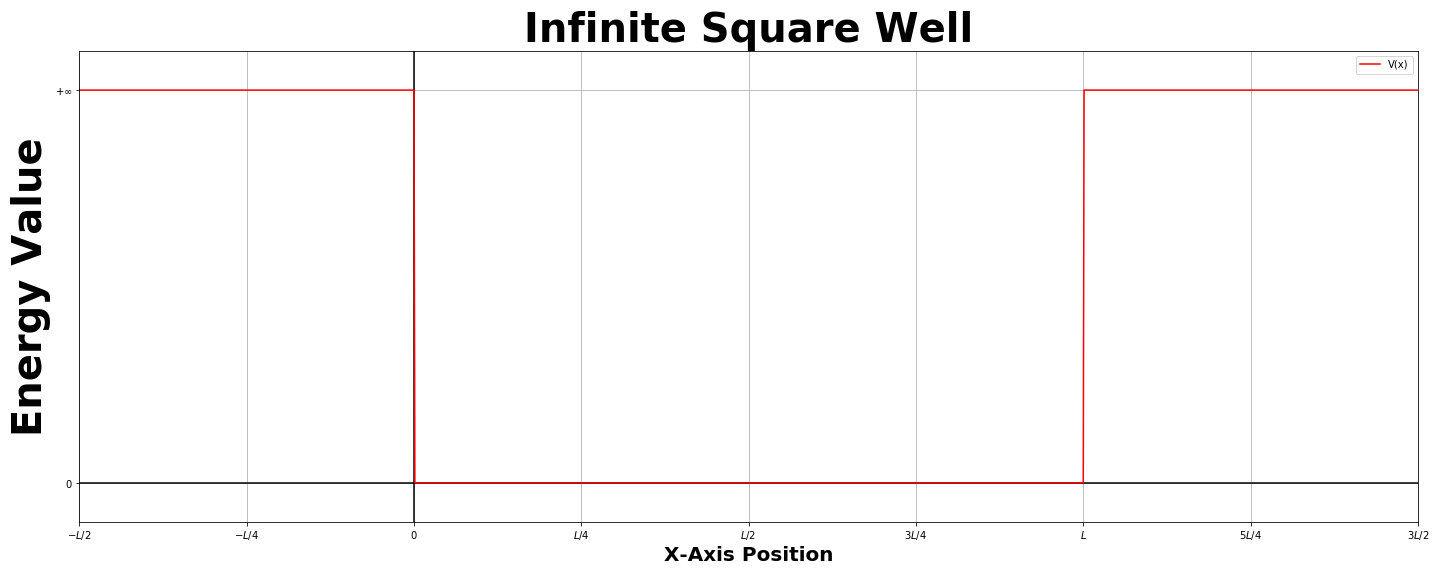
\includegraphics[scale=0.32]{ISW}
\end{center}
\paragraph*{}Right off of that bat, this allows for some great simplifications. First off, no matter what, Our particle cannot exist in the region $x < 0$ or $x > L$ because of the infinite amount of energy required to get there. Therefore, this quantum mechanical particle can \textit{only} exist in the region $0 \leq x \leq L$. With this, can can focus all of our attention to this region of space. All of the rules outline in the previous chapters still apply, but now we only have this small region of space to worry about.

% ================================

\subsection*{Solving the System 'By Hand'}

\paragraph*{}For the region between $x = 0$ and $x = L$, the TISE reads:
\begin{equation}
\label{ISW TISE}
-\frac{\hbar^2}{2m}\frac{d^2 \psi}{dx^2} = E\psi
\end{equation}
Notice how the $V(x)\psi(x)$ term from equation (\ref{1D TISE}) is gone because $V(x) = 0$ in these bounds. Now, we actually have much simpler equation to solve. We can use some algebraic manipulation to rearrange equation (\ref{ISW TISE}) into something very familiar from classical physics.
\begin{equation}
\label{HO ODE}
\frac{d^2 \psi}{dx^2} = -\frac{2mE}{\hbar^2}\psi
\end{equation}
\paragraph{}This is the standard ordinary differential equation for a mass-spring or any sort of harmonic oscillator -like system. This comes up all of the time in classical physics and is usually formed by equating Newton's second law, to Hooke's Law of ideal springs.  For simplicity's sake, lets make the assertion that a new constant can be created: $k = \frac{\sqrt{2mE}}{\hbar}$. (Note that is relies on the assumption that $E$ must be a positive value.) This changes the differential equation to:
\begin{equation}
\frac{d^2 \psi}{dx^2} = -k^2\psi
\end{equation}
Which has the solution:
\begin{equation}
\psi(x) = \alpha e^{+ikx} + \beta e^{-ikx}
\end{equation}
Which thanks to \textit{Euler's Identity}, can be rewritten as:
\begin{equation}
\psi(x) = a \sin(kx) + b \cos(kx)
\end{equation}
\paragraph*{}Here, $a$ and $b$ are constants chose based on initial condition or boundary conditions. From chapter 1, we learned that the wave function, 
$\psi(x)$ must be continuous over all space, and must be continuously differentiable over all of space. Since the potential function itself is not continuous differentiable (i.e. is peicewise defined), we can break this second rule. Regardless, since $\psi(x<0) = 0 $, and $\psi(x > L) = 0$, we can impose the boundary conditions on our system such that $\psi(x=0) = 0$ and $\psi(x=L) = 0$.
\paragraph*{}Applying these boundary conditions:
\begin{equation}
\psi(0) = a \sin(0) + b \cos(0) 
\text{\hspace*{8mm} and \hspace*{8mm}}
\psi(L) = a \sin(kL) + b \\cos(kL)
\end{equation}
Because of the nature of the sine and cosine functions, the only way for these equations to hold true is one of two ways. If $a = b = 0$, the whole wave function becomes $\psi(x) = 0$ which is a valid solution to the PDE, but not normalizeable, thus conflicts with one of our rules. Hence, the other option, just $b = 0$ is the valid conclusion. The resulting wave function for the infinite square well of width $L$ is:
\begin{equation}
\psi(x) = a \sin(kx) = a \sin\Big(\frac{\sqrt{2mE}}{\hbar}x\Big)
\end{equation}
\begin{flushright}
Where $kx$ must be an integer multiple of $\pi$: $kx = \pm \pi , \pm 2\pi , \pm 3\pm , ... , \pm n\pi , ...$ 
\end{flushright}
\paragraph*{}Because of the rotational symmetry of sine, ($-\sin(\theta) = +\sin(\theta)$), the negative integers become redundant, and since the function must fit "neatly" into a region $L$, the distinct solutions to the problem become:
\begin{equation}
\label{ISW spatial solution}
\psi_n(x) = A\sin \Big( \frac{n\pi}{L}x \Big)
\end{equation}
\paragraph*{}These $n$ functions are the \textit{energy eigenstates} to this problem and can be notated with kets: $\psi_n(x) = \ket{\psi_n}$. The constant that normalizes this ket is $ A = \sqrt{\frac{2}{L}}$. Just as presribebed by the equivalent eigenvalue problem, each eigenstate is appropriately orthonormal to the other eigenkets. Note that because we have eliminated all imaginary numbers, each ket is also it's own complex conjugate.
\begin{equation}
\braket{\psi_n}{\psi_m} = \frac{2}{L}\int_0^L \
\sin\big( \frac{n\pi x}{L} \big) \sin\big( \frac{m\pi x}{L} \big) dx =
\delta_{n,m}
\end{equation}
\begin{flushright}
Recall that $\delta_{n,m}$ returns $1$ if $n = m$ and $0$ if $n \neq m$.
\end{flushright}
\paragraph*{}Since we know have a collection of infinitely many eigenkets, we must also find each energy - eigenvalue as well - $E_n$. Since we know that $\frac{n\pi}{L} = \frac{\sqrt{2mE}}{\hbar}$, we can algebraically solve for $E_n$ and see that:
\begin{equation}
\label{energy for ISW}
E_n = \frac{n^2 \pi^2 \hbar}{2mL^2}
\end{equation}
\paragraph*{}Now we have a complete set of energy - eigenstates, given by $\ket{\psi_n}$ and all the corresponding energy - eigenvalues, given by $E_n$. Note that there are in infinite amount of both and perfectly match one - to - one. Every unique state has a unique energy and vice-versa. Finally, complete our analytical solution, we can form a linear combination all of our states. This the full solution to the infinite square well of width L is given by:
\begin{equation}
\label{ISW Full Solution}
\Psi(x,t) = \sqrt{\frac{2}{L}} \sum_n^{\infty} 
c_n \sin \Big( \frac{n\pi x}{L} \Big)
e^{-i\big( \frac{n^2 \pi^2}{2mL^2} \big)t}
\end{equation} 
\paragraph*{}Where $L$ is the width of the square well, $n$ is the energy level of the particle, and $m$ is the mass of the particle.

% ================================

\subsection*{Solving the System Numerically}
\textbf{Be sure to Check the Mathematical Appendix for note on how to build the Hamiltonian operator for some arbitrary potential!}

% ================================================================


\section{The Finite Square Well}

% ================================

\section{Multiple Square Wells}


% ================================

\section{The Harmonic Oscillator}


% ================================

\section{The Free Particle}


% ================================

\section{The Delta Function}


% ================================


% ================================================================
% ================================================================

\chapter{The Rules of the Game}

\paragraph*{}Just like any other subject, game or endeavor, quantum physics has a great many rules that go along with it. Be already outlined a great deal of these rules from a mathematical context, but this is not what I mean. Sure we can talk about how the same rules of linear algebra, differential equations and calculus all play roles in the physics, but getting bogged down in the math would be a great disservice. Instead, we'll call the rules of the game more like "formalisms" or "extra notes" on some of the topics that we've discovered already.

% ================================================================

\section{Observables and Hermitian Operators}

\paragraph*{}Operators are a huge part of quantum physics. They allow us to both conceptually and mathematically gather so much information about a quantum state. For example, if we had some quatum system described the the ket 
$\ket{\psi_\alpha}$, and then we wanted to know the total energy of this system, we just act on it with the Hamiltonian operator $\hat{H}$. Even if we don't know \textit{exactly} how this operator works, or it's composition in a linear algebra context, we know that the quantity:
\begin{equation}
E_\alpha = \hat{H}\ket{\psi_\alpha}
\end{equation}
is the total energy of the state $\ket{\psi_\alpha}$.
\paragraph*{}Furthermore, without anything anything else, we can find the \textit{average} total energy of the system across a linear combination of quantum states, $\ket{\Psi}$, would be given by:
\begin{equation}
\label{expect-val}
\expval{E} = \int \Psi^* \hat{H} \Psi dx = \bra{\Psi}\hat{H}\ket{\Psi}	
\end{equation}
\paragraph*{}Any operator that returns a \textit{physical} measurement on a state such as position, momentum, or energy is called an \textit{observable}. This concept is very important because being an operator also being an observable implies some extraneous conditions. We could for instance define some arbitrary operator, $\hat{Q}$, that returns some undetermined or unimportant quantity of our state. This operator comes with no external consequences- the value or values returned can be essentially anything.
\paragraph*{}Observables on the other hand, require that any measurements returned from them be \textit{real} values. Intutively, this makes a lot of sense, because we cant have an imaginary or complex measurement for average energy, it just doesn't make sense. Imaginary numbers are brilliant and useful mathematical tools for handling waves and oscillations and so many other topics, but in the real world, they aren't physical values. So, the outcome of a physical measurement, but be a physically realistic value, it must be real. So if $\hat{Q}$ is some arbitrary observable operator, then:
\begin{equation}
\label{observable}
\expval{\hat{Q}} = \expval{\hat{Q}}^* 
\end{equation}
\paragraph*{}This also forces us to recall some properties about Dirac notation. We know equation (\ref{observable}) is true, and the expectation value of an operator is given by (\ref{expect-val}), furthermore, the complex-conjugate of an inner product reverses the bra and kets with in. Thus:
\begin{equation}
\bra{\Psi}\hat{Q}\ket{\Psi} = 
\Big(\bra{\Psi}\hat{Q}\ket{\Psi}\Big)^* = 
\Big(\bra{\Psi}\hat{Q}\Big)\ket{\Psi} = 
\bra{\hat{Q}\Psi}\ket{\Psi}
\end{equation}
\paragraph*{}This property must hold true for all wave functions and states. An operator that is an observable has this very unique property. We can extend this property even a step further here, and define something called a \textit{Hermitian Operator}, which has an additional requirement:
\begin{equation}
\bra{\Psi_a}\Big(\hat{Q}\ket{\Psi_b}\Big) = 
\Big(\bra{\Psi_a}\hat{Q}\Big)\ket{\Psi_b}
\end{equation}
\paragraph*{}The operator acting in either direction produces the same result. Any operator that has all of these properties, is then a Hermetian operator. \textbf{In quantum physics, all observables are given by Hermitian operators.}

% ================================================================

\section{Commutivity}
\paragraph*{}In mathematics, operations can have the property of commutivity: that is: they commute. This means, that the order that they are applied to each other, or to another object is irrelevant to the outcome of that procedure. For example, multiplication is the most common and intuitive example of this. If we have three scalar values, $a$ and $b$, the order that they are multiplied- that is the order that they \textit{operate} on one another does not change the outcome. the product $a(b)$ is identical to the product $b(a)$. Thus the difference between them is zero.
\paragraph*{}In linear algebra and matrix multiplication, this is not always the case. Matrix $A$ acting on matrix $B$ may not not always be the same as matrix $B$ operating on matrix $A$: thus they do not commute. So we have the property: $AB \neq BA$. There are some very specific exceptions to thus rule, but more often than not in practice, matrices will not commute.
\paragraph*{}If two matrices - or in quantum physics, two \textit{operators} commute, the their commutivity is said to be zero. We test this relationship with the \textit{commutivity operator} defined below for two arbitrary operators $\hat{Q}$ and $\hat{R}$:
\begin{equation}
\label{commutator operator}
\comm{\hat{Q}}{\hat{R}} \equiv \hat{Q}\hat{R} - \hat{R}\hat{Q}
\end{equation}
All this operator does is return the difference between the order of the operators acting on some state. If the operator returns zero, then $\hat{Q}$ and $\hat{R}$ commute. If the result is non-zero, the operators do not commute. From this commutator, we can also establish some important rules for the operator. For any operator , $A$, $B$ and scalar $\alpha$, $\beta$:
\begin{multicols}{2}
\begin{itemize}
\item[•]\textbf{Self Commutivity:}\\
$ \comm{A}{A} = 0$
\item[•]\textbf{Commutivity with Scalars:}\\
$\comm{\alpha}{A} = 0$
\item[•]\textbf{Anti-symmetry:}\\
$ \comm{A}{B} = -\comm{B}{A} $
\item[•]\textbf{Hermitian Conjugates:}\\
$\comm{A}{B}^\dagger  = \comm{B^\dagger}{A^\dagger} $

\columnbreak

\item[•]\textbf{Factorization of Scalars:}\\
$\comm{\alpha A}{B} = \alpha \comm{A}{B}$
\item[•]\textbf{Distributive across addition:}\\
$\comm{A+B}{C} = \comm{A}{C} + \comm{B}{C}$
\item[•]\textbf{Multiplication:}\\
$\comm{AB}{C} = A\comm{B}{C} + \comm{A}{C}B$
\item[•]\textbf{Multiplication:}\\
$\comm{A}{BC} = \comm{A}{B}C + B\comm{A}{C}B$
\end{itemize}
\end{multicols}
Many of these rules can be extended to include nested commutation relations and various interactions with scalars and other mathematical objects.
\paragraph*{}The role of the commutator operator is very important in quantum physics, and will especially carry us through our discussion of uncertainty. It also gives rise to some helpful relations, most notably the \textit{canonical uncertainty relation} that relates the position and momentum operators:
\begin{equation}
\comm{\hat{x}}{\hat{p}} = \hat{x}\hat{p} - \hat{p}\hat{x} = i\hbar
\end{equation}


% ================================================================

\section{More on the Statistical Interpretation}

% ================================================================

\section{The Uncertainty Principle}
\paragraph*{}The concept of uncertainty has become the poster child for quantum physics. No doubt that before you knew a single bit of quantum of even classical mechanics, you had probably heard someone tell you about this radial concept of being able to know either position or momentum of a quantum system - but \textit{never} both. This idea is so counter intuitive and stands out because of that so maybe it's forgivable that so many people see this as one of defining characteristics of the field.
\paragraph*{}In reality, uncertainty really is a large part of quantum, any one the reasons that Schrodinger's theory was met with such distaste back in the 20th century. Even Albert Einstein who developed our models of special and general relativity thought the idea to be preposterous. The topic of uncertainty however, goes much farther than just not being able to know position and momentum together, but it really does shape our understanding of quantum physics - at least at this level.
\paragraph*{}Just like we discussed in chapter 1, all of our intuition of the macroscopic world is confirmed by our ability to take accurate and definite measurements. If we want to know position at any time, we can take a series of sample st regular time intervals to build some function to describe it as some $x(t)$. We can then compute our velocity , $v(t)$, and multiply it by our mass , $m$, and there we have it! Classical physics allows us to take a series of measurement that can give us our \textit{absolute} position and out \textit{absolute} momentum at any time. Thus we know them without any uncertainty, provided we have accurate measurements, our position and momentum values. But this is not simply a problem of instrumentation, we can't just hire a physicist or engineer to design a better machine to measure the quantities because uncertainty is a problem baked into the laws of nature.



% ================================================================

\section{More on Bases and Measurements}

% ================================================================

% ================================================================
% ================================================================

\chapter{The Next Level: \\ Spin and Angular Momentum}
\paragraph*{}The discussion of angular momentum 

% ================================================================
% ================================================================

\chapter{Mathematical Index}

% ================================================================


\section{Building the Hamiltonian Operator Numerically}
\paragraph*{}At the end of the first chapter, we discussed how the Time-Independent Schrodinger Equation can also be interpreted an an Energy - Eigenvalue problem. Rather than building a complicated algorithm to solve a partial differential equation, we can use an algorithm to solve an eigenvalue problem of a matrix instead. Although this conflicts with our new intuition about operators being more of continuous object as oppose to discrete matrices, the logistics of numerical problem solving still remains at hand - all objects must be discrete. In this section, we're going to discuss how to numerically build the Hamiltonian matrix.
\paragraph*{}I will use a mixture of psuedo-coding and written logic to express the steps to completing this task. Because of it current relevance in the scientific community, and readability, I will be using Python 3 and it's module \textit{numpy} for all explicit lines of code. Note than I will include a great deal of step-by-step comments so that you can repeat this procedure outside of Python 3.

% ================================

\subsection*{The Hamiltonian Revisited}

\paragraph*{}First, recall our energy eigen-equation:
\begin{equation}
\label{energy-evp}
\hat{H}\ket{\psi} = E\ket{\psi}
\end{equation}
And recall that the Hamiltonian operator acting on the state $\ket{\psi}$ can be written as the sum of the kinetic and potential energy operators acting on the state $\ket{\psi}$:
\begin{equation}
\hat{H}\ket{\psi} = \hat{T}\ket{\psi} + \hat{V}\ket{\psi}
\end{equation}
\paragraph*{}Using the same logic as building the Hamiltonian, we can build both the kinetic and potential energy operators independently, add them together, and then compute their eigenvalue problem.
\paragraph*{}Lets begin the process by defining some variables and setting some parameters. The exact value of $\hbar$ and the exact mass of electrons are both \textit{very} small numbers. In lower level programming languages and even in Python, entering these values exactly may cause rounding or estimation all sorts of other errors to arise, so we do something quite common in physics - we naturalize our units to the particular problem. We're going to set the value of both $\hbar$ and $m$ to be identically $1$.
\paragraph*{}While this may seem like cheating, we have to remember that these numbers may have values of $1$, but dimensionally, still have units of energy times time, and mass respectively. Since units are technically arbitrary, and the computer doesn't care about them anyway, this is a very value thing to do. In the end, this will save us a great deal of floating-point estimation errors and computational time. (For example $\hbar^2$ has a values somewhere around $1.11 \times 10^{-68}$ Joule-seconds in SI units) When we go back, we can always multiply our outputs by some constant to scale them back up into metric or imperial units as well.
\paragraph*{}In addition to setting units, and importing the numpy module, we need to determine the size of our matrix, which will be square. Both the kinetic energy potential energy parameters will also use this dimension, $N$, so it's important to define it early for consistency. We also need to create the one dimesions array to represent out space, as well as set bounds for that space.  So the first few lines of our program look like:
\begin{verbatim}
>>> import numpy as np
>>> hbar = 1                    # set h/2pi to be 1
>>> m = 1                       # set mass of electron to 1
>>> N = 2048                    # number of points in our space
>>> bnd = 10                    # set bounds on space
>>> x = np.arange(-bnd,+bnd,N)  # create the x-axis space
\end{verbatim}
Note that I have chosen $N$ to be 2048 because computers tend to like to work with integer exponents of $2$. What $N$ does is determine how many points we will divide outspace up into. This choice is somewhat arbitrary, in practice you can set it how you please. A larger number means a larger matrix- We will get $N$ eigenkets and $N$ eigenvalues. However, the computational time and complexity increases with the square of $N$.

% ================================

\subsection*{Kinetic Energy Operator}

\paragraph*{}The quantum kinetic energy operator (not acting on any state) is defined as:
\begin{equation}
\label{T}
\hat{T} = \frac{1}{2m}\hat{p}^2 = -\frac{\hbar^2}{2m} \frac{\partial^2}{\partial x^2}
\end{equation}
\paragraph*{}So, in order to build $\hat{T}$. We need to express (\ref{T}) as a \textit{matrix}. The constant out front, $-\frac{\hbar^2}{2m}$, is simple to handle, and since it's a matrix, we technically can treat it as that, multiplied by a matrix of all ones if left alone. So what we instead need it a matrix that can take some array, and return it's \textit{second} derivative. We'll call this matrix $\hat{D_2}$ or $D2$ is code-speak. To do this:

% ================================

% ================================================================


% ================================================================
% ================================================================

\end{document}